\documentclass[12pt,A4]{book}
\title{MIDILC:  A MIDI Language Compiler for Programmatic Music Composition}
\author{Alex ``Akiva'' Bamberger \\ Benjamin Mann \\ Fredric Lowenthal \\ Ye Liu}
\date{}

\usepackage{graphicx}
\usepackage[margin=1in]{geometry}
\begin{document}
\maketitle
\newpage
\tableofcontents
\newpage
\chapter{Introduction}
The language, hereafter referred to as MIDILC (pronounced MIDDLE C, standing for MIDI
Language Compiler), allows programmers to compose music. It compiles into MIDI format and
has syntax that is similar to Java, changing the basic primitives and the meaning of various
operators (Fig \ref{fig:types_in_midilc}).
\begin{figure}
\center
\begin{tabular}{|p{.2\textwidth}|p{.5\textwidth}|}
\hline
\verb|Number| & a value between $-2^{31}$ and $2^{31}-1$\\ \hline
\verb|Note| & a musical note with pitch and duration \\ \hline
\verb|Chord| & stores notes with equal durations and start times, represented by an integer list \\ \hline
\verb|Sequence| & a sequence of notes and chords, represented by a list of integer lists \\ \hline
\verb|+, -| & increase or decrease duration of notes; append to chords or sequences \\ \hline
\verb|.+, .-| & increase or decrease pitch of notes \\ \hline
\end{tabular}
\caption{Types and selected operators in the MIDILC language. }
\label{fig:types_in_midilc}
\end{figure}

The langauge is dynamically typed. Types must be used upon variable declaration, but are left optional for function declarations and arguments. Each type can be safely cast up in the following order: \verb|Number| $\rightarrow$ \verb|Note| $\rightarrow$ \verb|Chord| $\rightarrow$ \verb|Sequence|. The standard library, written in the language itself, supports major and minor chords, arpeggios, repetition, and other such basic and often used concepts. Note durations are specified in terms of whole notes (w), halves (h), quarters (q), eigths (e), and sixteenths (s). Sequences can either be appended to, which advances the ``current time'' by however long the appended sequence is, or else something can be inserted into a sequence at a given offset using subscripting. Functions are specified in the same way as in C.

Sequences and Chords can be output to the intermediate representation (IR) of CSV format using the play() function. In order to actually write the MIDI files, the CSV is fed to a Java program that interprets the CSV using the javax.sound.MIDI package.

Composing music on a computer is often done using GUIs that allow the user to drag and drop notes or using instrument inputs. This lets the musician hear his compositions as he is creating them, and often gives the musician a simple MP3 or MIDI ouput. As computer scientists, the MIDILC team finds such methods tedious, extraneuous and requiring too much natural music talent. MIDILC appeals to the virtues of any great programmer: laziness, hubris, and impatience \footnote{Wall, Larry. \textit{Programming Perl}, O'Reilly 2000.} and propose a language for those wishing to turn their quantitative skills into beautiful music.

MIDILC also attempts to redress other issues of regular music composition. Songs often have frequent recurring themes. Manually reusing these themes requires precision and dedication. If pieces of a song could be manipulated automatically for reuse and slight modification, song production speed could increase dramatically. The MIDILC language allows programmers to algorithmically generate notes, chords, and sequences of notes and chords by writing functions. This allows for writing interesting compositions that minimize time spent rewriting basic MIDI manipulation routines and implementing primitive musical constructs. The language works optimally with compositions that make consistent use of simple motifs as it encourages reuse of simple mathematical operations on notes and chords. 

MIDILC is tailored for crafting melody sequences. For a sequence containing a series of whole notes, one could easily manipulate the notes in the melody to create sequences of counterpoints to the melody. Using MIDILC, a \verb|major()| and \verb|minor()| function are easy to craft and chords simple to arpeggiate to make counterpoint. MIDILC allows for the simple concatenation and composition of sequences, and so complicated sequences could be easily made from simple starting blocks.

\chapter{Language Tutorial}
MIDILC was designed with the programmer in mind, but uses all the musical notation familiar to the musician. The lanuage is robust enough to fully support the idiomatic construction of Notes and Chords, as well as set tempo and note duration using \verb|Note| and \verb|Number| literals.
\section{An Introduction}
MIDILC is a C-like language used for generating midi music algorithmically. Each source file, with the extension .m, should contain a main() method. Like C, each line of code should be terminated with the semicolon.
\begin{verbatim}
main() {
    some_function();
\end{verbatim}

MIDILC’s basic types are Number, Note, Chord, and Sequence, the last three of which can be written into .midi files and played. All variables must be declared, one at a time, before they are called.

Numbers, the most basic type in MIDILC, supports integer values from $-2^{31}$ to $2^{31}-1$ MIDI instruments and notes.

\begin{verbatim}
Number num; /*declares the variable num */
num = 4; /* sets num to 4 */
num = num + 1; /* increment num by 1, 
                  so that it is now the value 5 */

/** The following snippet will provide a Note, the simplest 
of the playable musical types. */

Note n; /* declares the variable n*/

n = A; /* sets n to the note A, which by default is in 
          the 3rd octave and a quarter note */

/** Notes can also be initiated with more options:*/
n = A4w; /* sets n to the note A, in the 4th octave, as a whole note */
n = A4w + 4; /* sets n to A in the 4th octave as a whole note, 
                adds 4 beats (a quarter note’s worth) to its duration */
n = A4w .+ 4; /* sets n to A in the 4th octave as a whole note, then 
                 increase its pitch by 4 half steps (to C sharp) */
\end{verbatim}

The next type, \verb|Chord|, can be constructed from scratch, or based on notes that already exist. Unlike Note, Chord objects must be initiated with the \verb|new_chord()| function. Notice that since the \verb|+=| operator is not supported, adding to a \verb|Chord| requires one to set the Chord to itself plus the added object.

\begin{verbatim}
Chord a;
Chord b;
Chord c;
Chord d;

a = new_chord(); /* initializes a Chord object that plays nothing */
b = new_chord(C, E, G); /* initializes b to be a C major chord in the 
                           (default) 3rd octave with (default) duration 
                            of a quarter note*/
c = new_chord(n); /* initializes c to be a chord containing Note n */
a = a + n; /* adds the note n to a, which previously contained nothing playable */
\end{verbatim}

Sequence objects can be thought of as a collection of Note, Chord, and other Sequence objects. Construction of new Sequence objects is similar to that of new Chord objects. Both Note and Chord objects can be added to a Sequence object, in any permutation.
\begin{verbatim}
Sequence s1; /* declares s1 */
Sequence s2; /* declares s2 */

s1 = new_sequence();  /* initializes s1; empty sequence */
s2 = new_sequence(); /* initializes s2; empty sequence */
s1 = s1 + C4e; /* adds a note to s1 (4th octave C, eighth note duration) */
s1 = s1 + R; /* adds a rest to s1 */
s2 = s2 + a; /* adds Chord object a to s2 */

s2 = s2 + b; /* adds Chord object b to s2 */
\end{verbatim}

Finally, to print Sequence objects to .midi, the \verb|play()|function is invoked. \verb|play()| takes as an argument a \verb|Sequence|. Multiple calls of \verb|play()| in the same file will result in many Sequences played at once.

\begin{verbatim}
play(s1); /* prints s1 out*/
play(s2); /* prints s2 out*/
\end{verbatim}

To compile the program that you have just written, type the following into the command line:

\begin{verbatim}
./midilcc sample_program.m [sample_program_output]
\end{verbatim}

The last parameter is optional; if not given, a default name consisting of the name of the .m file with a .csv extenion will be given to the output CSV file. The compiler will print out any errors that may have occurred, and if the compilation was successful, a .csv file and a .midi file will be created in the same directory as the .m file. Simply open the .midi file with any media player to play it.

\section{Twinkle Twinkle Little Star}

The following tutorial will guide you through a simple program written in MIDILC, which produces a .midi file of the familiar tune “Twinkle Twinkle Little Star”. The full code can be found in the appendix.
	
The source files of MIDILC are saved as .m text files. First, create a .m file; call it twinkle.m. We 
will have one function, namely the \verb|main()| function, for all the code in this program. We declare the 
\verb|main()| function, and declare all the variables used, one per line:	

\begin{verbatim}
/* twinkle twinkle little star*/

/** Function declaration for main(), necessary for
    each MIDILC file */
Void main(){
  /** Declare variables */
  Chord ch1;
  Chord ch2;
  Chord ch3;
  Sequence s;
  Number i;
  Number r1;
  Number r2;
  
  /** Initialize chords */
  ch1 = new_chord(C,E,G);
  ch2 = new_chord(C,F,A);
  ch3 = new_chord(G3s,B3s,D4s,F4s);
  
  /** Initialize sequence */
  s = new_sequence();
 
  /** Build sequence up */
  s = s + C + C;
  s = s + ch1 + ch1 + ch2 + ch2 + ch1;
  
  s = s + arpeggiate(ch3) + F + F;
  
  s = s + E + E + D + D + C;
  
  set_tempo(125);
  
  play(s);
}

/** Function declaration for arpeggiate */
Sequence arpeggiate(Chord chord)
{
    /* declare variables */
    Number chord_length;
    Number i;
    Sequence s;

    /* build sequence */
    s = new_sequence();
    chord_length = chord.length;
    for(i = 0; i < chord_length; i=i+1)
    {
        s = s + chord[i];
    }
    return s;
}
\end{verbatim}

Congratulations, you have just written your first MIDILC program! To compile the program, invoke the MIDILC compiler (midilcc), as  described in the previous section.

\chapter{Language Reference Manual}

MIDILC is a C-like language that makes it simpler to algorithmically generate music.  It simplifies MIDI music creation by allowing programmers to specify song information in musical terms and write functions that process existing musical information.  By building off of simpler musical functions, such as arpeggios and chords, complex musical compositions can easily be programmed.

To eliminate the programming complexities from the MIDILC language, it has limited scope and data management capabilities.  MIDILC can be used following an imperative or functional paradigm and reduces hassle for the programmer by forcing static scope.

It compiles into MIDI files that can then be played in any standard media player.

\section{Lexical Conventions}
\begin{figure}
\center
\includegraphics[width=.75\textwidth]{notes.png}
\label{fig:pitches_and_notes}
\caption{The correspondence of notes and pitches in MIDI. }
\end{figure}
\subsection{Tokens}
Tokens consist of identifiers, keywords, constants, operators, and separators.  As with C, MIDILC is a free-form language and all white space characters are ignored (with the exception of separating tokens), as braces are used to identify the start and end of code blocks and semicolons are used to end statements.
\subsection{Comments}
/* and */ are used to indicate a block of comments (C-style comments).  There are no C++-style comments in MIDILC.
\subsection{Identifiers}
These are sequences of letters, digits, and underscores, starting with a letter or underscore.  Identifiers cannot be of the format \verb|[A-G R][b|\#\verb|]?[0-9]?[w h q e s]?|, as these are reserved for \verb|Note| literals.
\subsection{Keywords}
MIDILC has very few keywords; these include the following:

\begin{tabular}{|c|c|}
\hline
Types & Control \\ \hline
\verb|Number| & \verb|return| \\ \hline
\verb|Note|	& \verb|continue| \\ \hline
\verb|Chord| & \verb|break| \\ \hline
\verb|Sequence|	& \verb|if| \\ \hline
\verb|Void|	& \verb|else| \\ \hline
	& \verb|while| \\ \hline
	& \verb|for| \\ \hline
\end{tabular}


\subsection{Constants/Literals}
MIDILC allows a user to construct \verb|Note|s using pitch and duration (as \verb|Number| types), or using a set of \verb|Note| literals, specified by the note letter, accidental (if any), MIDI octave, and a letter that indicates the note’s duration (optional, and defaulting to a quarter note).  Duration can be specified by w (for whole note), h (for half note), q (for quarter note), e (for eigth note), and s (for sixteenth note).  Rests are indicated by using R instead of a note. Any \verb|Note| object constructed using a pitch with illegal properties will result in an error. \verb|Chord|s can easily be expressed using built-in chord generation function calls on \verb|Note| literals.  In addition, \verb|Number| literals also exist (integral numbers limited to signed 32-bit range).  MIDILC does not have floating-point literals.
Note that literals look like the following:
\verb|Ab7|,
\verb|C4s|,
\verb|G5h|

Pitches and \verb|Number| literals have the correspondence shown in figure \ref{fig:pitches_and_notes}.

\section{Meaning of Identifiers}
Identifiers in MIDILC have the following attributes: scope, name space, linkage, and storage duration. Since static scope is handled automatically, there are no storage class specifiers in MIDILC.
\subsection{Disambiguating Names}
\subsubsection{Scope}
The scope of of an identifier is defined as the region of a program within which it is visible, and begins when it is declared. In MIDILC, all identifiers are globally scoped, and are therefore visible to all blocks within a program unless hidden in another scope. This is due to the fact that the language automatically handles static identifiers.
\subsubsection{Name Space}
All the identifiers in MIDILC are categorized as ordinary identifiers. These include user-defined type names, object names, and function names.
\subsubsection{Linkage of Identifiers}
Identifiers in MIDILC may be linked across different files of the same program, but the identifier name must be unique in all files. Furthermore, the compiler will generate a compile time error about the identifier if there is a conflict.
\subsubsection{Storage Duration}
Storage duration denotes the lifetime of an object. All objects in MIDILC are static, and have static storage duration. The initialization of these objects occurs only once, prior to any reference.
\subsection{Object Types}
The MIDILC language supports two types of objects: numbers and musical notations.  Objects are dynamically typed.  Typing of an identifier is determined on assignment.
\subsubsection{Number type}
The only supported numerical type is \verb|Number|, which has a size of 32 bits and ranges from $-2^{31}$ to $2^{31} - 1$.  This is also the underlying type for all fields within the musical types.
\subsubsection{Musical types}
\verb|Note|, \verb|Chord|, and \verb|Sequence| are all of the musical types supported by MIDILC. \verb|Note| literals are  made up of strings consisting of integers and characters in sequences that match the following regular expression:
\verb|[A-G R][b |\#\verb|]?[0-9]?[w h q e s]?|
As these types are not stored directly internally, their sizes are not exact. As a general rule, for non-empty objects,
\verb|Number < Note < Chord < Sequence| in terms of their relative sizes.
\paragraph{Note type}
\verb|Note| type has the following attributes: pitch and duration. Pitch refers to the frequency of the note (Fig \ref{fig:pitches_and_notes}), and duration is specified as a type of note: whole, half, quarter, eighth, or sixteenth.  \verb|Note| literals with the pitch indicated as R instead of A-G are rests (numerically represented as -1).
\paragraph{Chord type}
\verb|Chord| type has the following attributes: duration and length. Duration is a \verb|Number| type that specifies a type of note: whole, half, quarter, eighth, or sixteenth. All \verb|Note| literals within the same \verb|Chord| must have the same duration.  This property can be specified as number of sixteenths. Length of the \verb|Chord| refers to the number of \verb|Note| literals in the \verb|Chord|.
\verb|Chord| literals can be constructed with the following syntax: \verb|new_chord(Note n1,  Note n2, Note n3);|
\paragraph{Sequence type}
\verb|Sequence| type has the following attributes: current and length. Each is of type \verb|Number|. Current denotes the current time where a new note will be inserted if a \verb|Note| or \verb|Chord| is added to this object. The length of the \verb|Sequence| refers to the number of \verb|Note| literals or \verb|Chord| objects in the \verb|Sequence|. Sequences can be constructed with the following command: \verb|new_sequence()|.
\subsubsection{Derived types}
\verb|Note|, \verb|Chord| and \verb|Sequence| objects can be derived. \verb|Note| can be derived from a \verb|Number| (specifying the pitch of the \verb|Note|, with duration of a quarter note). A \verb|Chord| be derived from a collection of \verb|Note| objects. A \verb|Sequence| can be derived from a collection of \verb|Note| or \verb|Chord| objects.
\subsubsection{Void type}
The \verb|Void| type specifies an empty set of return values. It never refers to an object.
\subsection{Objects and lvalues}
An object is a manipulable region of storage. An lvalue is an expression referring to an object, for example, an identifier.  Assignment causes the region of memory specified by the lvalue to be replaced or modified according to the value on the right side of the assignment.  For instance, if \verb|a = b| and \verb|c = b|, if \verb|b| is changed, \verb|a| and \verb|b| will remain unchanged.
\section{Operator Conversions}
Due to the nature of the primitive types, very few conversions are supported in MIDILC. It is possible to cast from \verb|Number| to \verb|Note|, from \verb|Note| to \verb|Chord|, from \verb|Note| to \verb|Sequence|, and from \verb|Chord| to \verb|Sequence|. Casts cannot be done in the opposite direction.
\subsection{Conversions of Number and Note}
\verb|Number| objects can be converted into \verb|Note| objects as a note with the pitch represented as an integer in MIDI notation. \verb|Note| objects cannot be converted to \verb|Number| objects. The new object has a default duration of quarter note.
\subsection{Conversions of Note and Chord}
\verb|Note| objects can be converted into \verb|Chord| objects as one-note chords. \verb|Chord| objects cannot be converted into \verb|Note| objects, as this is a narrowing conversion. The resulting \verb|Chord| has the same duration as the \verb|Note| used to construct it.
\subsection{Conversions of Note and Sequence}
\verb|Note| objects can be converted into \verb|Sequence| objects as a sequence that contains a single note. \verb|Sequence| objects cannot be converted into \verb|Note| objects, as this is a narrowing conversion, even if the \verb|Sequence| contains only a single \verb|Note|.
\subsection{Conversions of Chord and Sequence}
\verb|Chord| objects can be converted into \verb|Sequence| objects as a sequence that contains a single chord. \verb|Sequence| objects cannot be converted into \verb|Chord| objects, as this is a narrowing conversion, even if the \verb|Sequence| contains only a single \verb|Chord|.
\section{Expressions and Operators}

In MIDILC, expressions include one or more operators and a number of operands that follow certain associativity rules. Operators may change the value of an operand or leave it alone. 

Expressions (Fig 3.2) can be used for assignment or other operations. Associativity of these assignments can be overrridden by parentheses (Fig 3.3). Associativity of operators followed the table shown in figure \ref{fig:order_of_operations}.

\begin{figure}
\center
\begin{tabular}{|c|c|}
\hline
$assignment\mbox{-}expression$  & \verb|note = Ab7| \\ \hline
$operation\mbox{-}expression$   & \verb|Ab7 .+ 4| \\ \hline
\end{tabular}
\label{fig:expressions}
\caption{Examples of expressions}
\end{figure}
\begin{figure}
\center
\begin{tabular}{|p{.25\textwidth}|c|p{.25\textwidth}|}
\hline
Expression & Result & Explanation \\ \hline
\verb|C7 .+ 4| & \verb|E7| & \verb|Note| with E7 pitch \\ \hline
\verb|3 + 2 * 4| & \verb|11| &	Regular assignment order (multiplication has tightest binding, then addition) \\ \hline
\verb|(3 + 2) * 4| &\verb|20| & Parentheses change order of operations \\ \hline
\verb|note = C7;| \verb|new_chord(note,| \verb|note .+ 4,| \verb|note .+ 7);| & \verb|Chord| of \verb|(C7, E7, G7)| & Addition operator has tightest binding, followed by the assignment operator \\ \hline
\end{tabular}
\label{fig:associativity}
\caption{Associativity overridden by use of parentheses.}
\end{figure}

\begin{figure}
\center
\begin{tabular}{|p{.2\textwidth}|p{.2\textwidth}|c|c|}
\hline
Tokens\\(From High to Low Priority) & Operators & Class & Associativity \\ \hline
Identifiers, constants, parenthesized expression & Primary expression & Primary	& \\ \hline
\verb|() [] .|	& Function calls, subscripting, direct selection & Postfix & L-R \\ \hline
\verb|id as Type| & Cast & Binary & L-R \\ \hline
\verb|* /| &	Times/Divide	& Binary &	L-R \\ \hline
\verb|.+ .-| &	DotPlus/DotMinus	& Binary &	L-R \\ \hline
\verb|+ -| &	Add/Minus	& Binary &	L-R \\ \hline
\verb|== !=| & Equality comparisons & Binary & L-R \\ \hline
\verb|< <= >= >| & Relational Comparisons & Binary & L-R \\ \hline
\verb|&&| &	Logical and	& Binary	& L-R \\ \hline
\verb.||.	& Logical or & Binary & L-R \\ \hline
\verb|=| &	Assignment  & 	Binary & R-L \\ \hline
\verb|,| & Comma & Binary & L-R \\ \hline
\end{tabular}
\label{fig:order_of_operations}
\caption{Order of operations for built in operators}
\end{figure}
\subsection{Primary Expressions}
\subsubsection{Identifiers}
An lvalue or function designator (discussed in Built-In Functions).
\subsubsection{Constants}
An object of constant value (discussed in Built-In Functions).
\subsubsection{Parenthesized Expressions}
Parenthesized expressions allow a user to change the order of operations. They are executed before the operations and can be used as part of a larger expression (Fig 3.3).
\subsection{Postfix}
Postfix calls are made as follows:

\begin{tabular}{|c|c|}
\hline
Function call & \verb|Chord c; c =  new_chord(Ab6, Ab7, C4);| \\ \hline
Subscripting & \verb|Note n; n = c[0];| \\ \hline
Direct selection &    \verb|Number i; i = n.pitch;| \\ \hline
\end{tabular}

\subsubsection{Function calls}
The syntax of a function call is as follows:

\begin{tabular}{l l}
$postfix\mbox{-}expression$ & $\rightarrow (argument\mbox{-}expression\mbox{-}list_{opt})$\\
$argument\mbox{-}expression\mbox{-}list$ & $\rightarrow argument\mbox{-}expression$\\
& $\rightarrow argument\mbox{-}expression\mbox{-}list, argument\mbox{-}expression$
\end{tabular}

An argument expression list may either be a single argument or a list of arguments. All functions are allowed to be recursive.
Each function must be declared before it is called. With that in mind, certain casts are made by the runtime compiler to match arguments. A \verb|Number| may be cast to a \verb|Note|, \verb|Chord|, or \verb|Sequence|, for example.
A function may only take the a parameter of type Void. For functions like this, a function call may include no parameters.

\subsubsection{Subscripting}
Certain objects may be acted upon by the subscripting operation. For example, a \verb|Chord| object may be acted upon by a subscript to select a particular note in the chord. Similarly, a \verb|Sequence| object may be acted upon to select a \verb|Chord| at any particular moment in time. For a \verb|Chord| object, the index of the subscript reflects the order that a \verb|Note| was added. For a \verb|Sequence| object, the index subscript indicates the order that Chords were inserted in.
The subscripting operator allows both retrieval and mutation of elements in those objects that support it. There is no implicit casting for subscription.

\subsubsection{Direct Selection}
Used to change pitch and duration in objects of type \verb|Note|, \verb|Chord|, or \verb|Sequence|. Pitch and duration are treated as objects of type  \verb|Number| with the pitch affected (either positively or negatively) by the successor operand. For example, \verb|C7.pitch = C7.pitch + 1| will result in C\#7.
Similarly for duration: \verb|C7.duration = C7.duration + 1| will result in C7 with a duration of a 1/16th note greater.
Direct selection can be done for the following parameters on the following objects:
\verb|Note|: pitch, duration
\verb|Chord|: duration, length
\verb|Sequence|: current, length.  
Note, however, that length cannot be used as an lvalue.

\subsection{Unary Operations}
\subsubsection{Casting}
Syntax of casting is as follows:

\begin{tabular}{l l}
$cast\mbox{-}expression$  & $\rightarrow unary\mbox{-}expression$ \\
& $\rightarrow (cast\mbox{-}expression$ as $type\mbox{-}name)$ 
\end{tabular}

Casting allows a user to explicitly change the Type of an object, according to the order established in Musical Types. Implicitly casting will take place during a function call or in the use of a binary operator between two objects of different type. If, however, we wanted to craft two notes, and then append one to another in a chord, we would need to do the following:
\verb|s = (((note1 as Chord) as Sequence) + note2)|
This would allow us to use the + operator of Sequences instead of the + operator of Notes.
\subsection{Binary Operations}

\subsubsection{Mult/Divide}
Used to multiply or divide two \verb|Number| objects.

Syntax is as follows:\\

\begin{tabular}{l l}
$mult\mbox{-}divide\mbox{-}expression$ & $\rightarrow argument\mbox{-}expression$ \\
& $\rightarrow mult\mbox{-}divide\mbox{-}expression * argument\mbox{-}expression$\\
& $\rightarrow mult\mbox{-}divide\mbox{-}expression / argument\mbox{-}expression$
\end{tabular}

\subsubsection{DotAdd/DotMinus}
Used to increment or decrease the pitch of a \verb|Note| object.

Syntax is as follows:\\

\begin{tabular}{l l}
$dot\mbox{-}plus\mbox{-}minus\mbox{-}expression$ & $\rightarrow argument\mbox{-}expression$ \\
& $\rightarrow dot\mbox{-}plus\mbox{-}minus\mbox{-}expression .+ argument\mbox{-}expression$\\
& $\rightarrow dot\mbox{-}plus\mbox{-}minus{-}expression .- argument\mbox{-}expression$
\end{tabular}

\subsubsection{Add/Subtract}
Used to add or subtract two \verb|Number| objects. When applied to objects of type \verb|Note|, \verb|Chord|, or \verb|Sequence|, results in a \verb|Sequence| object with given elements concatenated. If two or more objects of different type are concatenated, the element of highest cast determines the cast. That is, a \verb|Note| added to a \verb|Sequence| would return a new \verb|Sequence| with the given note appended as a degenerate \verb|Chord| to the end.

Syntax is as follows:\\

\begin{tabular}{l l}
$add\mbox{-}expression$ & $\rightarrow cast\mbox{-}expression$ \\
& $\rightarrow add\mbox{-}expression + cast\mbox{-}expression$\\
& $\rightarrow add\mbox{-}expression - cast\mbox{-}expression$
\end{tabular}

\subsubsection{Relational comparisons}
Yields a \verb|Number| result (1 if true, 0 if false). Allows for comparison between objects (casting is done in one direction).

\begin{tabular}{l l}
$relational\mbox{-}expression$  & $\rightarrow add\mbox{-}expression$\\
& $\rightarrow relational\mbox{-}expression < add\mbox{-}expression$ \\
& $\rightarrow relational\mbox{-}expression > add\mbox{-}expression$ \\
& $\rightarrow relational\mbox{-}expression <= add\mbox{-}expression$ \\
& $\rightarrow relational\mbox{-}expression >= add\mbox{-}expression$ \\
\end{tabular}

\subsubsection{Equality comparisons}
Compares two values for equality. MIDILC uses the number 0 to denote false and all values other than 0 to denote truth. Equality follows the following rules:
Two \verb|Number| objects are equal if they evaluate to the same value
Two \verb|Note| objects are equal if they have the same pitch and duration
Two \verb|Chord| objects are equal if they have the same notes and the same duration
Two \verb|Sequence| objects are equal if they have the same chords in the same order

\begin{tabular}{l l}
$equality\mbox{-}expression$  & $\rightarrow relational\mbox{-}expression$\\
& $\rightarrow equality\mbox{-}expression$ == $relational\mbox{-}expression$\\
& $\rightarrow equality\mbox{-}expression$ != $relational\mbox{-}expression$\\
\end{tabular}

\subsubsection{Logical and}
Performs a logical ``and'' on two expressions. Returns 0 if the left expression evaluates to 0. Otherwise, evaluates right expression. If true, returns 1; if false, 0.
Syntax:

\begin{tabular}{l l}
$logical\mbox{-}AND\mbox{-}expression$  & $\rightarrow logical\mbox{-}OR\mbox{-}expression$\\
& $\rightarrow logical\mbox{-}AND\mbox{-}expression$ \verb|&&| $logical\mbox{-}OR\mbox{-}expression$
\end{tabular}

This is done with lazy evaluation.
\subsubsection{Logical or}
Performs a logical ``or'' on two expressions. Returns 1 if ever the left expression evaluates to 1. Otherwise, evaluates right expression. If true, 1; if false, 0.
Syntax:

\begin{tabular}{l l}
$logical\mbox{-}OR\mbox{-}expression$  & $\rightarrow logical\mbox{-}AND\mbox{-}expression$\\
& $\rightarrow logical\mbox{-}OR\mbox{-}expression $ \verb.||. $ logical\mbox{-}AND\mbox{-}expression$
\end{tabular}

This is again an example of MIDILC’s power to perform lazy evaluation.
\subsubsection{Assignment}
Right associative. The expression on the right is evaluated and then used to set the lvalue. The rvalue must have the same type as the lvalue; no casting is implicitly done.
\subsubsection{Comma}
Separates elements in a list (such as parameters in a function or \verb|Note| literals in a \verb|Chord|). Example of \verb|Chord| constructor:
\verb|Chord myChord;| \verb|myChord = new_chord(C4, E4);|
\section{Declarations}
Declarations specify the interpretation given to a set of identifiers.

\begin{tabular}{l l}
$direct\mbox{-}declarator$ & $\rightarrow type\mbox{-}specifier$ $declarator$
\end{tabular}

Only a single declarator can be declared at once.  Declarators must be preceded by the type of the identifier.  At most one declaration of the identifier can appear in the same scope and name space.  
\subsection{Storage class specifiers}
Static scope is handled automatically because functions have access to any identifiers not declared in their scope. No storage class specifiers are available.
\subsection{Type specifiers}
Type specifiers listed below.  Syntax as follows:

\begin{tabular}{l l}
$type\mbox{-}specifier$  & \verb|Void| \\
& \verb|Number|\\
& \verb|Note|\\
& \verb|Chord|\\
& \verb|Sequence|
\end{tabular}

\subsection{Type qualifiers}
Types cannot be declared mutable or immutable by the programmer.  All types are mutable.
\subsection{Function Declarators}
There are no function prototypes (all function declarations are definitions).  The syntax for function declarators is shown below:

\begin{tabular}{l l l}
$direct\mbox{-}declarator $ & $\rightarrow (identifier\mbox{-}list_{opt})$ { $body$ } \\
$identifier\mbox{-}list$  & $\rightarrow identifier\mbox{-}list,$ $direct\mbox{-}declarator$
\end{tabular}

For example,
$T$ $D$ $(identifier\mbox{-}list_{opt})$
creates a function with identifier D and return type T with the specified parameters. An identifier list declares the types of and identifiers for the formal parameters of a function.

Function declarators do not support variable additional arguments.  

If the type of any parameter declared in the identifier list is other than that which would be derived using the default argument promotions, an error is posted.  Otherwise, a warning is posted and the function prototype remains in scope.

When a function is invoked for which a function is defined, no attempt is made to convert each actual parameter to the type of the corresponding formal parameter specified in the function prototype. Instead an error is thrown.  

The following is an example of a function definition:
\verb|Chord transposeChord(Chord oldChord,| \verb|Note newKey) { ... }|
This declares a function \verb|transposeChord()| which returns a \verb|Chord| and has two parameters: a \verb|Chord| and a \verb|Note|.  
\subsection{Initialization}
A declaration of a type can specify an initial value for the identifier after being declared.  The initializer is preceded by = and consists of an expression.

\begin{tabular}{l l}
$initializer$ & $\rightarrow assignment\mbox{-}expression$\\
\end{tabular}

Variables that are not explicitly initialized may cause a null pointer exception during compilation. When an initializer applies to a literal, it consists of a single expression, perhaps in parentheses.  The initial value of the object is taken from the expression.  Type conversion is only attempted with an explicit cast.

\subsubsection{Examples of initialization}
\begin{verbatim}
Note root;
Chord notes;
Sequence gProgression;
/*Initializes root with a note literal.*/
root = C3q;

/*Initializes notes with a chord literal*/
notes = new_chord( root, root .+ 4, root .+ 7 );

/*Initializes gProgression with the result of the function call.*/
gProgression = oneFourFiveProg( G7q );
\end{verbatim}
\section{Statements}
A statment is a complete instruction to the midi compiler. Except as indicated, statements are executed in sequence.  Statements have the following form:

\begin{tabular}{l l}
$statement$ & $\rightarrow expression\mbox{-}statement$\\
& $\rightarrow selection\mbox{-}statement$\\
& $\rightarrow iteration\mbox{-}statement$\\
& $\rightarrow jump\mbox{-}statement$\\
\end{tabular}

\subsection{Expression statement}
Most statements are expression statements, which have the following form:

\begin{tabular}{l l}
$expression\mbox{-}statement$ & $\rightarrow expression;$
\end{tabular}

Usually expression statements are expressions evaluated for their side effects such as assignments or function calls.
\subsection{Compound statement or block}
A compound statement (or block) groups a set of statements into a syntactic unit.  The set can have its own declarations and initializers, and as the following form:

\begin{tabular}{l l}
$compound\mbox{-}statement$  & $\rightarrow \{declaration\mbox{-}list$ $statement\mbox{-}list_{opt}\}$\\
$declaration\mbox{-}list$ & $\rightarrow declaration$\\
& $\rightarrow declaration\mbox{-}list$ $declaration$\\
$statement\mbox{-}list$  & $\rightarrow statement$\\
& $\rightarrow statement\mbox{-}list$ $statement$\\
\end{tabular}

Declarations within compound statements have block scope.  If any of the identifiers in the declaration list were previously declared, the outer declaration is hidden for the duration of the block, after which it resumes its force.  Function declarations can only be defined at the outermost scope.
\subsection{Selection statements}
Selection statements include the if and else statements and have the following form:

\begin{tabular}{l l}
$selection\mbox{-}statement$ & $\rightarrow if$ $(expression)$ $statement$\\
& $\rightarrow if$ $(expression)$ $statement$ $else$ $statement$
\end{tabular}

Selection statements choose one of a set of statements to execute, based on the evaluation of the expression.  The expression is referred to as the controlling expression.
\subsubsection{if statement}
The controlling expression of an \verb|if| statement must have \verb|Number| type. For both forms of the \verb|if| statement, the first statement is executed if the controlling expression evaluates to nonzero.  For the second form, the second statement is executed if the controlling expression evaluates to zero.  An else clause that follows multiple sequential else-less if statements is associated with the most recent \verb|if| statement in the same block (that is, not in an enclosed block).
\subsection{Iteration statements}
Iteration statements execute the attached statement (called the body) repeatedly until the controlling expression evaluates to zero.  In the for statement, the second expression is the controlling expression.  The format is as follows:

\begin{tabular}{l l}
$iteration\mbox{-}statement$ & $\rightarrow while(expression)$ $statement$\\
& $\rightarrow for$ $(expression;$ $expression$ $;$ $expression)$ $statement$
\end{tabular}

The controlling expression must have \verb|Number| type.
\subsubsection{while statement}
The controlling expression of a \verb|while| statement is evaluated before each execution of the body.
\subsubsection{for statement}
The for statement has the form specified above.  The first expression specifies the initialization for the loop.  The second expression is the controlling expression, which is evaluated before each iteration.  The third expression often specifies incrementation.  It is evaluated after each iteration. It is equivalent to the following:

\begin{tabular}{l l}
$expression\mbox{-}1$  & $\rightarrow while$ $(expression\mbox{-}2)$ $\{statement$ $expression\mbox{-}3\}$\\
\end{tabular}

One exception exists, however.  If a \verb|continue| statement is encountered, $expression\mbox{-}3$ of the \verb|for| statement is executed prior to the next iteration.
\subsection{Jump statements:}

\begin{tabular}{l l}
$jump\mbox{-}statement$ & $\rightarrow$\verb|continue|\\
                & $\rightarrow$\verb|break|\\
                & $\rightarrow$\verb|return| $expression_{opt};$
\end{tabular}

\subsubsection{continue statement}
The \verb|continue| statement can appear only in the body of an iteration statement.  It causes control to pass to the loop-continuation portion of the smallest enclosing \verb|while| or \verb|for| statement; that is, to the end of the loop.
\subsubsection{break statement}
The \verb|break| statement can appear only in the body of an iteration statement or code attached to a switch statement. It transfers control to the statement immediately following the smallest enclosing iteration, terminating its execution.
\subsubsection{return statement}
A function returns to its caller by means of the \verb|return| statement. The value of the expression is returned to the caller as the value of the function call expression. The \verb|return| statement cannot have an expression if the type of the current function is \verb|Void|.
If the end of a function is reached before the execution of an explicit \verb|return|, an implicit \verb|return| (with no expression) is executed. If the value of the function call expression is used when none is returned, the behavior is undefined.

\section{Built-In Functions}

\begin{tabular}{l p{.4\textwidth}}
\verb|Void play(Sequence s)| & Instructs compiler to write a \verb|Sequence| to the MIDI file.\\
\verb|Void set_tempo(Number n)| & Sets the tempo of the file to \verb|Number|.\\
\verb|Void set_instrument("instrument")| & Sets the instrument for the song\\
\verb|Sequence new_sequence()| & Initializes an empty \verb|Sequence|.\\
\verb|Chord new_chord(Note n1, Note n2, ...)| & Initializes a \verb|Chord| object.\\
\verb|Number rand(Number n)| & Returns a random number between 0 and \verb|n|.\\
\end{tabular}

\chapter{Project Plan}
\section{Development Process}
The team met once a week on Sundays to set milestones and deadlines as well as discuss progress and set design goals. The language was first designed using a collaborative approach, using whiteboards to brainstorm and Google Docs to save notes.

The team used an SVN repository hosted on Google Code to store code. Development was done using open source text editors, including vim, Eclipse, and gedit. Code was written in OCaml for the compiler and in Java for the Assembler. The Intermediate Representation (IR) for the code was in CSV format, which was created by executing the bytecode. Team members updated the repository at the end of each development session. E-mail and Google Docs were used for realtime collaboration.

With a few exceptions each module was accompanied with tests written by the module's author. Team members were expected to supply both a test and an expected output, which could be used to verify the success of a test by each team member. Scripts were written to quickly test the code and compare it to the standard.
\section{Style Guide}
A general style guide was used by the team during development.
\subsection{O'Caml source}
\begin{itemize}
\item Variables named using lowercase letters, with spaces replaced by underscores.
\item Types named using lowercase letters with spaces replaced by underscores (e.g. \verb|program|, \verb|expr|)
\item Tokens named using uppercase letters without spaces (e.g. \verb|TYPE|, \verb|NOTE|)
\item Constructors named using Camel Case (e.g. \verb|Binop|, \verb|Num|)
\item Modules named using uppercase first letter, lowercase rest (e.g. \verb|Ast|, \verb|Bytecode|)
\item 2 spaces for each tab
\item Comments about specific implementation details using (* single asterisk comment *)
\item Comments about general implementation details using (** double asterisk comment *)
\item Meaningful variable names for all global variables (e.g. \verb|note_map|, \verb|jumps|)
\item Fewer than 140 character per line (viewable without runoff with window maximized)
\item Keep lines aligned
\end{itemize}
\subsection{Java source}
\begin{itemize}
\item Kept all tests in \verb|src/components/| folder
\end{itemize}
\subsection{MIDILC source}
\begin{itemize}
\item Named all variables and functions with lowercase first letters
\item Added a multi-line C style comment (/** */) at the top of each class
\item Named classes with `.m' extension (for MIDILC)
\item Declared all variables at top of each method
\end{itemize}
\subsection{Testing}
\begin{itemize}
\item Kept all tests in \verb|src/tests/| folder
\item Named all tests with gold standards with prefix ``test-''
\item Named all output files for gold standard tests with .out
\end{itemize}
\section{Project Timeline}
\begin{tabular}{l p{.5\textwidth}}
11/20 & Finish project plan and arch design sections of final report\\
      & Mostly complete scanner, top level, and AST\\
11/27 & Each person should have finished at least one unit test that works for his component\\
      & Make major headway on parser and compiler\\
12/4 & Finish testing plan\\
12/11 & Finish overall system (source should compile into MIDI files)\\
12/18 & Finish up final sections of report\\
\end{tabular}
\section{Roles and Responsibilities}
\subsection{Akiva Bamberger}
Designed initial structure of typing system and operators. Wrote parts of proposal and LRM. After working on the initial scanner and AST (of a statically typed prototype), worked to build the modules for the dynamically typed language Ben developed while working on executer and compiler. Worked on modules included printing sequences to the correct CSV output, constructing new chord objects, adding break and continue, and allowing users to treat the language as statically typed. Improved the bytecode, improved the implementation of some operators, and wrote many tests, working with Fred and Ye. Edited and wrote many parts of the final report.

\subsection{Ben Mann}
Worked with Fred to set up project milestones and start writing the final report.  Wrote proposal and sections 5 and 6 of the LRM.  Starting with MICROC, implemented the major features of the language, including the dynamic typing system, most of the operators; in other words, the necessary parts of the toplevel, scanner, AST, parser, compiler, and executor.  Designed and implemented the bytecode representation.  Wrote the first tests in the language for the basic features and wrote the first script to turn a file from MIDILC code into a .wav file that could be listened to for accuracy.  After the language compiled, distributed tasks to other team members and taught them how the type system and other details were implemented.

\subsection{Fred Lowenthal}
My contributions to the written portions of the project were contributing to the proposal and LRM, and planning and writing parts of the final report 

In terms of contributions to the project development, I worked on the initial parser (though many changes were made afterwards).  I also modified the assembler to handle setting instruments and tempo, through the programming and requisite research.  I also implemented some parts of the compiler and executor (and several necessary parser/AST/lexer/bytecode changes as necessary) for the tempo and instrument functions, along with adding the requisite String literal type.  I also finished implementing several operators.
\subsection{Ye Liu}
Worked on the proposal and LRM. Worked with Fred on the assembler, modifying it and taking out extra MIDI detais that are out of the scope of MIDILC. Wrote test cases for library functions (most scales), and some newer features (multiply). Worked on assembling the final report.

\section{Languages and Tools Used}
The team used O'Caml, Java, and bash scripting to complete the langauge. The tools used included: gedit and Vim for editing O'Caml; Eclipse for editing Java; and gedit for editing bash scripts. The javax.swing.midi library proved most useful for transcribing MIDI from CSV. A CSV2MIDI library was also used, originally authored by Stephen Steffes (http://www.penguinpeepshow.com/CSV2MIDI.php). timidity, a .midi-to-.wav converter, was used to convert .wav files from the MIDI output by the assembler. A Google code hosted SVN repository was used for version control. E-mail and Google Docs were used to share documentation.

\section{Project Log}
\subsection{SVN Activity}
\subsubsection{Size of directories}
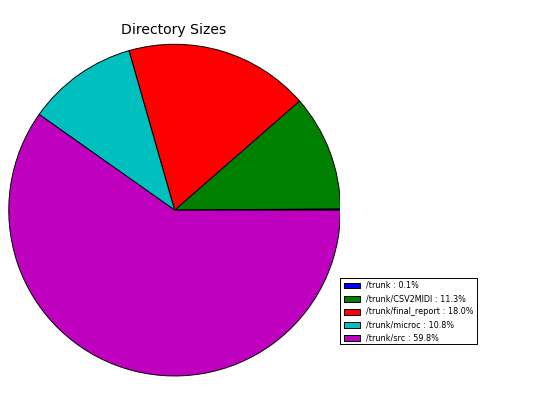
\includegraphics[width=.8\textwidth]{svngraphs/dirsizepie.png}
\subsubsection{Size of code as a function of time}
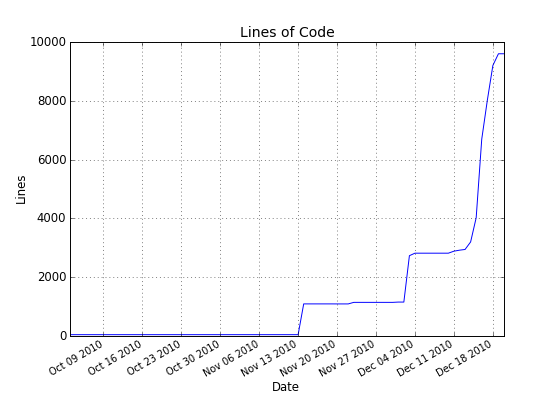
\includegraphics[width=.8\textwidth]{svngraphs/loc.png}
\subsubsection{Actions by time of day}
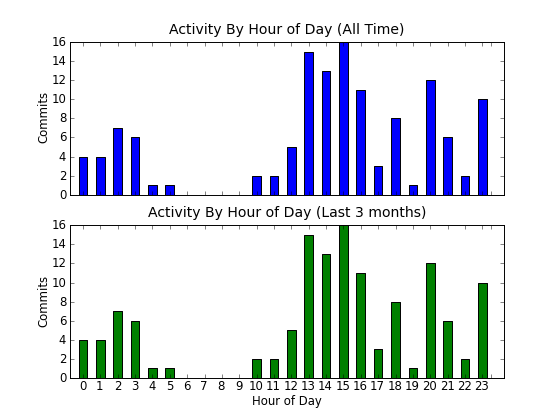
\includegraphics[width=.8\textwidth]{svngraphs/actbytimeofday.png}

\subsection{SVN Log}
\begin{verbatim}
------------------------------------------------------------------------
r137 | Akiva.Bamberger | 2010-12-20 00:10:37 -0500 (Mon, 20 Dec 2010) | 2 lines

Final Report!

------------------------------------------------------------------------
r136 | Akiva.Bamberger | 2010-12-19 23:37:11 -0500 (Sun, 19 Dec 2010) | 2 lines

Updated final report. Working on final tidbits.

------------------------------------------------------------------------
r135 | Akiva.Bamberger | 2010-12-19 21:25:13 -0500 (Sun, 19 Dec 2010) | 3 lines

Updated final reports.


------------------------------------------------------------------------
r134 | 8enmann@gmail.com | 2010-12-19 19:37:14 -0500 (Sun, 19 Dec 2010) | 2 lines

Added graphical statistics on svn commit history.

------------------------------------------------------------------------
r133 | 8enmann@gmail.com | 2010-12-19 15:34:01 -0500 (Sun, 19 Dec 2010) | 3 lines

updated


------------------------------------------------------------------------
r132 | 8enmann@gmail.com | 2010-12-19 14:51:42 -0500 (Sun, 19 Dec 2010) | 2 lines

Fixed some formatting, added some TODOs, and added role/responsibility for me.

------------------------------------------------------------------------
r131 | yeliu2428@gmail.com | 2010-12-19 14:36:26 -0500 (Sun, 19 Dec 2010) | 1 line

Did some formatting. Added Fred's section 7 contributions.
------------------------------------------------------------------------
r130 | yeliu2428@gmail.com | 2010-12-19 14:14:25 -0500 (Sun, 19 Dec 2010) | 1 line

Updated blockdiagram.png to have a white background (so we can see what the hell is going on.)
------------------------------------------------------------------------
r129 | yeliu2428@gmail.com | 2010-12-19 10:56:58 -0500 (Sun, 19 Dec 2010) | 1 line

Added to Section 6, testing
------------------------------------------------------------------------
r128 | yeliu2428@gmail.com | 2010-12-19 10:45:43 -0500 (Sun, 19 Dec 2010) | 1 line

formatted 2.2, Twinkle Twinkle. Still kinda funky looking.
------------------------------------------------------------------------
r127 | yeliu2428@gmail.com | 2010-12-19 05:12:28 -0500 (Sun, 19 Dec 2010) | 3 lines

Added in 2.2 (Twinkle Twinkle);
Corrected Fred's name spelling;
Still need to format Twinkle Twinkle more.
------------------------------------------------------------------------
r126 | 8enmann@gmail.com | 2010-12-19 04:39:29 -0500 (Sun, 19 Dec 2010) | 3 lines

Corrected an error in variable declaration in the LRM.


------------------------------------------------------------------------
r125 | Akiva.Bamberger | 2010-12-19 00:29:32 -0500 (Sun, 19 Dec 2010) | 3 lines

Tutorial (by Ye) added to code


------------------------------------------------------------------------
r124 | Akiva.Bamberger | 2010-12-19 00:05:18 -0500 (Sun, 19 Dec 2010) | 2 lines

Changes made to add "Roles and Responsibilities"

------------------------------------------------------------------------
r123 | Akiva.Bamberger | 2010-12-18 23:56:52 -0500 (Sat, 18 Dec 2010) | 2 lines

Made changes to get log on the right lines...

------------------------------------------------------------------------
r122 | Akiva.Bamberger | 2010-12-18 23:55:31 -0500 (Sat, 18 Dec 2010) | 3 lines

Made changes to code to comply with style guidelines.


------------------------------------------------------------------------
r121 | Akiva.Bamberger | 2010-12-18 23:37:04 -0500 (Sat, 18 Dec 2010) | 2 lines

Updated the final report

------------------------------------------------------------------------
r120 | Akiva.Bamberger | 2010-12-18 21:02:03 -0500 (Sat, 18 Dec 2010) | 2 lines

Cleaned up the LRM; trucking along with Ye.

------------------------------------------------------------------------
r119 | yeliu2428@gmail.com | 2010-12-18 18:12:00 -0500 (Sat, 18 Dec 2010) | 2 lines

added block diagram.png

------------------------------------------------------------------------
r118 | 8enmann@gmail.com | 2010-12-18 16:54:40 -0500 (Sat, 18 Dec 2010) | 2 lines

Made a few comments, but there's a lot of formatting to fix and info to update.

------------------------------------------------------------------------
r117 | Akiva.Bamberger | 2010-12-18 16:51:20 -0500 (Sat, 18 Dec 2010) | 2 lines

Incrementally better.

------------------------------------------------------------------------
r116 | Akiva.Bamberger | 2010-12-18 16:15:43 -0500 (Sat, 18 Dec 2010) | 2 lines

Added stairway to heaven, first part.

------------------------------------------------------------------------
r115 | yeliu2428@gmail.com | 2010-12-18 01:52:25 -0500 (Sat, 18 Dec 2010) | 1 line

Added test for inequality
------------------------------------------------------------------------
r114 | yeliu2428@gmail.com | 2010-12-18 01:21:35 -0500 (Sat, 18 Dec 2010) | 1 line

Added test for multiply
------------------------------------------------------------------------
r113 | 8enmann@gmail.com | 2010-12-17 20:47:48 -0500 (Fri, 17 Dec 2010) | 2 lines

Slightly modified dvorak test.

------------------------------------------------------------------------
r112 | yeliu2428@gmail.com | 2010-12-17 20:46:40 -0500 (Fri, 17 Dec 2010) | 1 line

Added test for natural minor scale creation.
------------------------------------------------------------------------
r111 | 8enmann@gmail.com | 2010-12-17 19:36:41 -0500 (Fri, 17 Dec 2010) | 3 lines

Added the most ballin' test ever.


------------------------------------------------------------------------
r110 | Fredmaster2 | 2010-12-17 17:47:14 -0500 (Fri, 17 Dec 2010) | 1 line

Implemented setting instruments via name in the assembler.  For backwards compatibility, numbers are still supported (using quotation marks)
------------------------------------------------------------------------
r109 | Akiva.Bamberger | 2010-12-17 16:26:42 -0500 (Fri, 17 Dec 2010) | 2 lines

A symphony of pi!

------------------------------------------------------------------------
r108 | 8enmann@gmail.com | 2010-12-17 15:03:23 -0500 (Fri, 17 Dec 2010) | 3 lines

French horn ftw.


------------------------------------------------------------------------
r107 | 8enmann@gmail.com | 2010-12-17 14:54:57 -0500 (Fri, 17 Dec 2010) | 2 lines

Updated test.

------------------------------------------------------------------------
r106 | 8enmann@gmail.com | 2010-12-17 14:47:51 -0500 (Fri, 17 Dec 2010) | 3 lines

Added multiply and divide.


------------------------------------------------------------------------
r105 | yeliu2428@gmail.com | 2010-12-17 14:24:27 -0500 (Fri, 17 Dec 2010) | 3 lines

Two things:
1. Changed the author info for the .java files in /components
2. Changed .csv files for the scale tests to .out files
------------------------------------------------------------------------
r104 | yeliu2428@gmail.com | 2010-12-17 13:41:56 -0500 (Fri, 17 Dec 2010) | 1 line

Added test-melodicminor
------------------------------------------------------------------------
r103 | yeliu2428@gmail.com | 2010-12-17 13:37:17 -0500 (Fri, 17 Dec 2010) | 1 line

Added test-harmonicminor
------------------------------------------------------------------------
r102 | yeliu2428@gmail.com | 2010-12-17 13:29:41 -0500 (Fri, 17 Dec 2010) | 1 line

Added test-majorscale to tests.
------------------------------------------------------------------------
r101 | Fredmaster2 | 2010-12-17 03:01:15 -0500 (Fri, 17 Dec 2010) | 1 line

Forgot to take QUOTE back out
------------------------------------------------------------------------
r100 | 8enmann@gmail.com | 2010-12-17 02:55:20 -0500 (Fri, 17 Dec 2010) | 2 lines

Fixed warning and some formatting.

------------------------------------------------------------------------
r99 | yeliu2428@gmail.com | 2010-12-17 02:50:58 -0500 (Fri, 17 Dec 2010) | 1 line

formatted midilc_report.tex with subsections and \verb tags
------------------------------------------------------------------------
r98 | Fredmaster2 | 2010-12-17 02:41:35 -0500 (Fri, 17 Dec 2010) | 3 lines

Implemented string literals for specifying instruments, and modified test and set_instrument function accordingly.

The assembler has not yet been updated, so the csv files produced with an instrument set will not currently work with the compiler
------------------------------------------------------------------------
r97 | 8enmann@gmail.com | 2010-12-17 00:12:36 -0500 (Fri, 17 Dec 2010) | 2 lines

Renamed a bunch of tests, added comments, and added attribution.

------------------------------------------------------------------------
r96 | Akiva.Bamberger | 2010-12-16 23:20:15 -0500 (Thu, 16 Dec 2010) | 2 lines

Updated tex file with latex

------------------------------------------------------------------------
r95 | yeliu2428@gmail.com | 2010-12-16 23:19:39 -0500 (Thu, 16 Dec 2010) | 1 line

added novice programs to final_report/novice. there's a program that generates a sequence (test-twinkle), one that generates a random sequence (test-randomseq), and one that generates a two-sequence file (test-doubleseq).
------------------------------------------------------------------------
r94 | Akiva.Bamberger | 2010-12-16 23:03:42 -0500 (Thu, 16 Dec 2010) | 5 lines

Added final report files.

Working with Ye on getting this pretty.


------------------------------------------------------------------------
r93 | Fredmaster2 | 2010-12-16 22:07:26 -0500 (Thu, 16 Dec 2010) | 1 line

Added note, chord, and sequence equality and inequality operators, and accompanying test
------------------------------------------------------------------------
r92 | Fredmaster2 | 2010-12-16 21:05:42 -0500 (Thu, 16 Dec 2010) | 1 line

Fixed PPQ issue - 16 to 4 (i.e. everything's 4x slower now)
------------------------------------------------------------------------
r91 | Akiva.Bamberger | 2010-12-16 20:56:50 -0500 (Thu, 16 Dec 2010) | 2 lines

Changed code to allow addition of two notes-- this results in the duration of the second being added on to the duration of the first.

------------------------------------------------------------------------
r90 | Akiva.Bamberger | 2010-12-16 20:21:20 -0500 (Thu, 16 Dec 2010) | 2 lines

Changed testall to fix problem with .m versus \.m (in regex)

------------------------------------------------------------------------
r89 | Fredmaster2 | 2010-12-16 20:16:29 -0500 (Thu, 16 Dec 2010) | 3 lines

Added lots of tests, and several new test cases

Added new TODO list in main src directory
------------------------------------------------------------------------
r88 | Akiva.Bamberger | 2010-12-16 20:10:01 -0500 (Thu, 16 Dec 2010) | 4 lines

Added comments to the code, as well as an output file for
test-recursion.


------------------------------------------------------------------------
r87 | Akiva.Bamberger | 2010-12-16 18:18:59 -0500 (Thu, 16 Dec 2010) | 18 lines

Added a script to let people make midi files out of .m files, like gcc.

The syntax is as follows:

./midilcc tests/test.m /music/song

This will create /music/song.midi and /music/song.wav.

Alternatively, someone can type

./midilcc tests/test.m

and it will create tests/test.midi and tests/test.wav.


-- Akiva


------------------------------------------------------------------------
r86 | Akiva.Bamberger | 2010-12-16 18:11:24 -0500 (Thu, 16 Dec 2010) | 5 lines

Added tests for recursion and added comments for break/continue.

Allowed using types in declarations.


------------------------------------------------------------------------
r85 | Fredmaster2 | 2010-12-16 12:17:36 -0500 (Thu, 16 Dec 2010) | 3 lines

Added number-based instrument_set and tempo_set assembler implementations (instrument lookup check not yet added).

Added set_instrument and set_tempo tests
------------------------------------------------------------------------
r84 | Akiva.Bamberger | 2010-12-16 03:16:22 -0500 (Thu, 16 Dec 2010) | 6 lines

Added break and continue.

Please look at these changes. Some things have been added to the code
to allow for breaks and continues to work as intended.


------------------------------------------------------------------------
r83 | Fredmaster2 | 2010-12-15 17:35:50 -0500 (Wed, 15 Dec 2010) | 3 lines

Changed set_tempo to add tempo_marker, and added set_instrument function (currently uses instrument number, need to add string to stack?)

These functions work, and pass tests, but the version of the assembler that supports them hasn't been committed yet
------------------------------------------------------------------------
r82 | 8enmann@gmail.com | 2010-12-15 03:43:01 -0500 (Wed, 15 Dec 2010) | 4 lines

Oops, realized I wasn't seeding the random generator.
Now the test SHOULD fail every time.  Teehee.


------------------------------------------------------------------------
r81 | 8enmann@gmail.com | 2010-12-15 03:40:14 -0500 (Wed, 15 Dec 2010) | 5 lines

Added rand(max) which returns an integer from 0 to max.
For some reason the test file has random notes but they come out the same
every time, even across compilation.  At least it's testable!


------------------------------------------------------------------------
r80 | 8enmann@gmail.com | 2010-12-15 03:13:27 -0500 (Wed, 15 Dec 2010) | 4 lines

Modified makefile so you can just type "make test" to run all the tests.
Also edited the test.sh script to make the gold standard of the correct filename format.
Added a missing gold standard for for4.

------------------------------------------------------------------------
r79 | 8enmann@gmail.com | 2010-12-15 03:00:21 -0500 (Wed, 15 Dec 2010) | 2 lines

added support for direct selection as lvalue and tests

------------------------------------------------------------------------
r78 | Akiva.Bamberger | 2010-12-15 02:34:28 -0500 (Wed, 15 Dec 2010) | 2 lines

Made changes to fix earlier submission. Added a test.

------------------------------------------------------------------------
r77 | 8enmann@gmail.com | 2010-12-15 02:32:18 -0500 (Wed, 15 Dec 2010) | 2 lines

restored pristine example files

------------------------------------------------------------------------
r76 | Akiva.Bamberger | 2010-12-15 01:39:23 -0500 (Wed, 15 Dec 2010) | 8 lines

This one's a killa.
1) Chords can now be created using the call new_chord 
   and can take variable number of args
2) You can now print a Chord directly
3) I really refrained from making the log just a goofy header
4) We can use what I did for new_chord on any future functions we want
   that take variable length args!

------------------------------------------------------------------------
r75 | 8enmann@gmail.com | 2010-12-15 00:39:20 -0500 (Wed, 15 Dec 2010) | 3 lines

Added fancy tests to TODO


------------------------------------------------------------------------
r74 | Fredmaster2 | 2010-12-14 22:07:17 -0500 (Tue, 14 Dec 2010) | 1 line

Added test-attribute gold standard and changed test.sh to not remove csv file (to make it easier to produce gold standards).
------------------------------------------------------------------------
r73 | Fredmaster2 | 2010-12-14 21:56:47 -0500 (Tue, 14 Dec 2010) | 1 line

Added gold standard output, removed interpret test from testall.sh, and wrote sequence test
------------------------------------------------------------------------
r72 | 8enmann@gmail.com | 2010-12-14 21:37:50 -0500 (Tue, 14 Dec 2010) | 2 lines

Added tests for attribute assignment, updated parser to resolve shift reduce conflict.

------------------------------------------------------------------------
r71 | 8enmann@gmail.com | 2010-12-14 20:01:08 -0500 (Tue, 14 Dec 2010) | 2 lines

Added support for attribute selection

------------------------------------------------------------------------
r70 | 8enmann@gmail.com | 2010-12-14 18:01:57 -0500 (Tue, 14 Dec 2010) | 2 lines

Syntax for l-value selection implemented... committing before implementing executor code.

------------------------------------------------------------------------
r69 | 8enmann@gmail.com | 2010-12-14 16:25:55 -0500 (Tue, 14 Dec 2010) | 4 lines

Implemented mod operator.
Cleaned up built-in function declaration in compiler.


------------------------------------------------------------------------
r68 | 8enmann@gmail.com | 2010-12-14 15:41:00 -0500 (Tue, 14 Dec 2010) | 4 lines

Deleted java files since they've been moved to /components.
Added test script and executable jar file.


------------------------------------------------------------------------
r67 | 8enmann@gmail.com | 2010-12-14 15:22:19 -0500 (Tue, 14 Dec 2010) | 2 lines

New tests added

------------------------------------------------------------------------
r66 | 8enmann@gmail.com | 2010-12-14 15:21:35 -0500 (Tue, 14 Dec 2010) | 2 lines

Moved java files, compiled, and made a manifest file

------------------------------------------------------------------------
r65 | Akiva.Bamberger | 2010-12-14 02:11:41 -0500 (Tue, 14 Dec 2010) | 2 lines

Implemented print_sequence
Changed the string_of_list and string_of_list_list to only take one arg



------------------------------------------------------------------------
r64 | Akiva.Bamberger | 2010-12-14 01:13:50 -0500 (Tue, 14 Dec 2010) | 2 lines

Added print_sequence

------------------------------------------------------------------------
r63 | 8enmann@gmail.com | 2010-12-13 15:42:50 -0500 (Mon, 13 Dec 2010) | 5 lines

Added support for adding chords to sequences.
Fixed tests to use new_sequence constructor.
Fixed new_sequence constructor.


------------------------------------------------------------------------
r62 | 8enmann@gmail.com | 2010-12-13 15:19:48 -0500 (Mon, 13 Dec 2010) | 3 lines

updated TODO


------------------------------------------------------------------------
r61 | 8enmann@gmail.com | 2010-12-13 14:58:52 -0500 (Mon, 13 Dec 2010) | 4 lines

Added sequence constructor function as a built-in.
Fixed sequence addition.


------------------------------------------------------------------------
r60 | 8enmann@gmail.com | 2010-12-13 12:34:45 -0500 (Mon, 13 Dec 2010) | 2 lines

Oops, forgot that chord start times have to be updated. Added a TODO.

------------------------------------------------------------------------
r59 | 8enmann@gmail.com | 2010-12-13 12:32:13 -0500 (Mon, 13 Dec 2010) | 3 lines

Added support for adding sequences together.


------------------------------------------------------------------------
r58 | 8enmann@gmail.com | 2010-12-12 21:44:07 -0500 (Sun, 12 Dec 2010) | 3 lines

GREAT SUCCESS. pipeline complete.
had to fix an infinite loop I accidentally created in handling Rts

------------------------------------------------------------------------
r57 | Akiva.Bamberger | 2010-12-12 21:15:11 -0500 (Sun, 12 Dec 2010) | 2 lines

Added some things!

------------------------------------------------------------------------
r56 | 8enmann@gmail.com | 2010-12-12 20:48:48 -0500 (Sun, 12 Dec 2010) | 2 lines

cleaned up formatting, killed some pointless code

------------------------------------------------------------------------
r55 | 8enmann@gmail.com | 2010-12-12 18:41:10 -0500 (Sun, 12 Dec 2010) | 2 lines

Killed java directory. Relevant java files should be placed in the src folder.

------------------------------------------------------------------------
r54 | 8enmann@gmail.com | 2010-12-12 18:37:46 -0500 (Sun, 12 Dec 2010) | 3 lines

Added LRM for reference, modified a comment in compiler.


------------------------------------------------------------------------
r53 | 8enmann@gmail.com | 2010-12-12 18:34:44 -0500 (Sun, 12 Dec 2010) | 4 lines

Implemented a lot of stuff in the executor and made the 
comments in bytecode.ml better.


------------------------------------------------------------------------
r52 | Akiva.Bamberger | 2010-12-12 14:43:14 -0500 (Sun, 12 Dec 2010) | 3 lines

To get simple tests to work again...


------------------------------------------------------------------------
r51 | 8enmann@gmail.com | 2010-12-12 13:53:52 -0500 (Sun, 12 Dec 2010) | 2 lines

Everything compiles

------------------------------------------------------------------------
r50 | 8enmann@gmail.com | 2010-12-12 02:26:48 -0500 (Sun, 12 Dec 2010) | 3 lines

Revamped everything.
Still have to add some cases to the pattern match in execute to make it compile.

------------------------------------------------------------------------
r49 | 8enmann@gmail.com | 2010-12-11 20:45:34 -0500 (Sat, 11 Dec 2010) | 3 lines

Everything compiles.  Do not commit if you can't run make!


------------------------------------------------------------------------
r48 | Fredmaster2 | 2010-12-11 20:07:47 -0500 (Sat, 11 Dec 2010) | 1 line


------------------------------------------------------------------------
r47 | 8enmann@gmail.com | 2010-12-11 20:06:28 -0500 (Sat, 11 Dec 2010) | 4 lines

Everything compiles except the toplevel because it needs the executor.
LOTS of things changed, mostly do to with how operators get passed around.
Still a lot to do.  Added comments in some of the places.  Threw errors for some unimplemented stuff.

------------------------------------------------------------------------
r46 | 8enmann@gmail.com | 2010-12-11 17:56:35 -0500 (Sat, 11 Dec 2010) | 2 lines

These files were corrupted. Restoring originals.

------------------------------------------------------------------------
r45 | 8enmann@gmail.com | 2010-12-04 16:33:12 -0500 (Sat, 04 Dec 2010) | 4 lines

Modified bytecode spec to use uniform types.  Still need to add type-specific operators.

Added a function to the compiler that converts note literals into tuples with pitch and duration as int * int tuples.

------------------------------------------------------------------------
r44 | 8enmann@gmail.com | 2010-12-03 16:44:01 -0500 (Fri, 03 Dec 2010) | 2 lines

Deleted interpreter.  Not making one. 

------------------------------------------------------------------------
r43 | 8enmann@gmail.com | 2010-12-03 16:43:15 -0500 (Fri, 03 Dec 2010) | 2 lines

Added toplevel for Ye to work on.

------------------------------------------------------------------------
r42 | Fredmaster2 | 2010-12-03 16:29:37 -0500 (Fri, 03 Dec 2010) | 1 line

Added execute and modified bytecode to add bytecode types.
------------------------------------------------------------------------
r41 | yeliu2428@gmail.com | 2010-12-03 16:23:13 -0500 (Fri, 03 Dec 2010) | 1 line

Moved assembler stuff.
------------------------------------------------------------------------
r40 | Akiva.Bamberger | 2010-12-03 16:01:20 -0500 (Fri, 03 Dec 2010) | 4 lines

Updated the parser and ast files.

Good job, friends!

------------------------------------------------------------------------
r39 | 8enmann@gmail.com | 2010-12-03 15:42:42 -0500 (Fri, 03 Dec 2010) | 3 lines

edited wrong bytecode file before. fixed.


------------------------------------------------------------------------
r38 | 8enmann@gmail.com | 2010-12-03 15:41:18 -0500 (Fri, 03 Dec 2010) | 2 lines

small edits

------------------------------------------------------------------------
r37 | yeliu2428@gmail.com | 2010-12-03 15:25:06 -0500 (Fri, 03 Dec 2010) | 1 line

Updated default time resolution to 960 ppq.
------------------------------------------------------------------------
r36 | yeliu2428@gmail.com | 2010-12-03 15:06:22 -0500 (Fri, 03 Dec 2010) | 1 line

Added CSV2MIDI2.java, which is modified from the CSV2MIDI directory to match our needs.
------------------------------------------------------------------------
r35 | 8enmann@gmail.com | 2010-12-03 13:58:24 -0500 (Fri, 03 Dec 2010) | 2 lines

moved type defs

------------------------------------------------------------------------
r34 | Fredmaster2 | 2010-12-03 13:57:27 -0500 (Fri, 03 Dec 2010) | 1 line

Fixed dot and bracket s/r error
------------------------------------------------------------------------
r33 | Akiva.Bamberger | 2010-12-03 13:45:51 -0500 (Fri, 03 Dec 2010) | 2 lines

Small changes made

------------------------------------------------------------------------
r32 | Fredmaster2 | 2010-12-03 13:45:06 -0500 (Fri, 03 Dec 2010) | 1 line

Added brackets and dot to parser
------------------------------------------------------------------------
r31 | 8enmann@gmail.com | 2010-12-03 13:44:02 -0500 (Fri, 03 Dec 2010) | 2 lines

small modifications to compiler and added microc interpreter

------------------------------------------------------------------------
r30 | Akiva.Bamberger | 2010-12-03 13:43:45 -0500 (Fri, 03 Dec 2010) | 2 lines

Did it

------------------------------------------------------------------------
r29 | 8enmann@gmail.com | 2010-12-03 13:33:06 -0500 (Fri, 03 Dec 2010) | 2 lines

Deleted repository testing files

------------------------------------------------------------------------
r28 | Akiva.Bamberger | 2010-12-03 13:22:16 -0500 (Fri, 03 Dec 2010) | 5 lines

Adding, my BFFs!

This Abstract Syntax Tree takes care of most things.


------------------------------------------------------------------------
r27 | 8enmann@gmail.com | 2010-12-03 13:18:43 -0500 (Fri, 03 Dec 2010) | 2 lines

Relevant parts should be modified as necessary and moved to /src

------------------------------------------------------------------------
r26 | Fredmaster2 | 2010-12-03 13:14:56 -0500 (Fri, 03 Dec 2010) | 1 line

Updated parser with types
------------------------------------------------------------------------
r25 | 8enmann@gmail.com | 2010-12-03 12:59:42 -0500 (Fri, 03 Dec 2010) | 4 lines

Added some necessary files, modified slightly from their MICROC originals.  Note the TODO file in tests, which contains a list of tests that need to be written as they are supported.
Tests can't be written until the whole pipeline up to the interpreter is somewhat complete.


------------------------------------------------------------------------
r24 | Akiva.Bamberger | 2010-12-03 12:48:38 -0500 (Fri, 03 Dec 2010) | 2 lines

Changed the way types are dealt with

------------------------------------------------------------------------
r23 | Fredmaster2 | 2010-12-03 11:44:05 -0500 (Fri, 03 Dec 2010) | 1 line

Added location change for parser.mly
------------------------------------------------------------------------
r22 | Akiva.Bamberger | 2010-12-03 11:30:58 -0500 (Fri, 03 Dec 2010) | 2 lines

Adding for Fred

------------------------------------------------------------------------
r21 | Fredmaster2 | 2010-12-01 20:55:12 -0500 (Wed, 01 Dec 2010) | 1 line

Worked on parser.mly, some changes need to be made to scanner for further work.
------------------------------------------------------------------------
r20 | Akiva.Bamberger | 2010-11-23 23:53:01 -0500 (Tue, 23 Nov 2010) | 2 lines

Adding to src (sorry, edited first in microc file)

------------------------------------------------------------------------
r19 | Akiva.Bamberger | 2010-11-23 23:19:11 -0500 (Tue, 23 Nov 2010) | 1 line


------------------------------------------------------------------------
r18 | Akiva.Bamberger | 2010-11-23 23:18:38 -0500 (Tue, 23 Nov 2010) | 1 line


------------------------------------------------------------------------
r17 | Akiva.Bamberger | 2010-11-23 23:17:43 -0500 (Tue, 23 Nov 2010) | 2 lines

First set of changes

------------------------------------------------------------------------
r16 | yeliu2428@gmail.com | 2010-11-20 18:35:49 -0500 (Sat, 20 Nov 2010) | 1 line

removed testing file from /src
------------------------------------------------------------------------
r15 | Fredmaster2 | 2010-11-14 14:47:08 -0500 (Sun, 14 Nov 2010) | 1 line

Added sample final report and milestones (current as of 11/14)
------------------------------------------------------------------------
r14 | Fredmaster2 | 2010-11-14 13:52:59 -0500 (Sun, 14 Nov 2010) | 1 line

Added the microc stuff
------------------------------------------------------------------------
r13 | Akiva.Bamberger | 2010-10-03 15:19:39 -0400 (Sun, 03 Oct 2010) | 1 line

What's up BAMF lovers
------------------------------------------------------------------------
r12 | Akiva.Bamberger | 2010-10-03 15:17:11 -0400 (Sun, 03 Oct 2010) | 1 line

Initial import.
------------------------------------------------------------------------
r11 | 8enmann@gmail.com | 2010-10-03 15:04:22 -0400 (Sun, 03 Oct 2010) | 1 line

asdf
------------------------------------------------------------------------
r10 | 8enmann@gmail.com | 2010-10-03 15:03:19 -0400 (Sun, 03 Oct 2010) | 2 lines

test

------------------------------------------------------------------------
r9 | 8enmann@gmail.com | 2010-10-03 15:01:27 -0400 (Sun, 03 Oct 2010) | 1 line

testing more
------------------------------------------------------------------------
r8 | 8enmann@gmail.com | 2010-10-03 14:59:15 -0400 (Sun, 03 Oct 2010) | 1 line

testing
------------------------------------------------------------------------
r7 | yeliu2428@gmail.com | 2010-10-03 14:58:30 -0400 (Sun, 03 Oct 2010) | 1 line

testing
------------------------------------------------------------------------
r3 | Akiva.Bamberger | 2010-10-03 14:22:47 -0400 (Sun, 03 Oct 2010) | 2 lines

Adding a file for source files...

------------------------------------------------------------------------
r2 | Akiva.Bamberger | 2010-10-03 14:06:58 -0400 (Sun, 03 Oct 2010) | 2 lines

Added the proposal

------------------------------------------------------------------------
r1 | (no author) | 2010-10-03 14:01:58 -0400 (Sun, 03 Oct 2010) | 1 line

Initial directory structure.
------------------------------------------------------------------------
\end{verbatim}
\chapter{Architecture \& Design}
\section{Block Diagram}

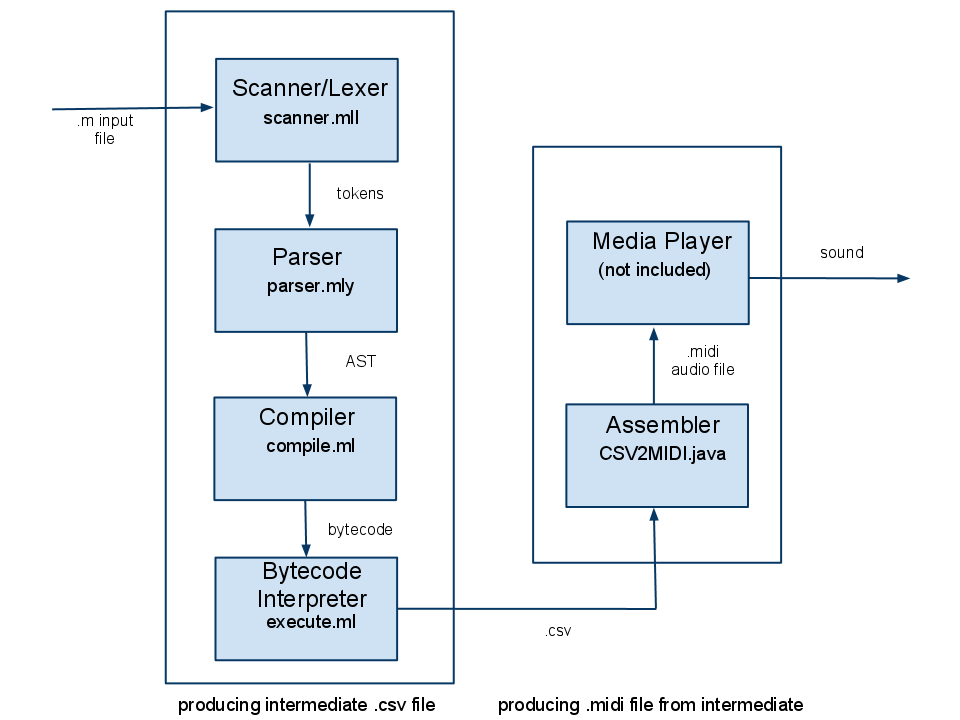
\includegraphics[width=\textwidth]{blockdiagram.png}

\section{Interface between components}
The input is a .m file written according to the LRM and the block diagram shown in the above figure. The input file is converted into tokens by the scanner/lexer, parsed into an abstract syntax tree, compiled into bytecode, and is further compiled into a CSV by the bytecode interpreter. Finally, the CSV file is assembled into a MIDI file by the Java-based assembler, which can then be played on any standard media player.  The two outputs generated by each .m source file is a .csv file containing CSV information, and a .midi file to be played.  All components are written in OCAML except for the assembler, which is written in Java.  The parser is generated by OCAMLYACC.  The media player is not included here and can be written in any language.

The MIDILC language logically consists of a lexer, parser, bytecode compiler, and assembler.  As the lexer reads in tokens, it invokes the parser.  At this point, syntax errors prevent the compiler from running and output an error.  When parsing is finished, the bytecode compiler is invoked, which generates a series of human-readable CSV bytecodes, which mimic the MIDI structure.  It is at this point that runtime errors (such as granularity issues or bounds check violation) are generated.  Finally, the assembler is run on the CSV to output a type Standard MIDI File.
\section{Who Implemented What}
Fred, Akiva, and Ben: Lexer, Parser, Bytecode, Executor, Compiler

\noindent Fred and Ye: Assembler

\noindent View the section on Project Log for more details.
\chapter{Test Plan}
\section{Representative Source}
\subsection{For Loop}
\subsubsection{Source Code}
\begin{verbatim}
/** Adds many notes to a sequence using a simple for loop */
main() {
  Note a; 
  Sequence b;
  Number i;
  b = new_sequence();
  a = Aq;
  for (i = 0 ; i < 12 ; i = i + 1) {
    b = b + a;
    b = b + ((a as Chord) + (a .+ i));
  }
  play(b);
}
\end{verbatim}
\subsubsection{Bytecode}
\begin{verbatim}
0 global variables
0 Jsr 2
1 Hlt
2 Ent 3
3 Jsr -3
4 Sfp 2
5 Drp
6 Not (69,4)
7 Sfp 1
8 Drp
9 Num 0
10 Sfp 3
11 Drp
12 Sjp (15,23,0)
13 Bra 21
14 Lfp 2
15 Lfp 1
16 Add
17 Sfp 2
18 Drp
19 Lfp 2
20 Lfp 1
21 Cst Chord
22 Lfp 1
23 Lfp 3
24 Dad
25 Add
26 Add
27 Sfp 2
28 Drp
29 Lfp 3
30 Num 1
31 Add
32 Sfp 3
33 Drp
34 Lfp 3
35 Num 12
36 Lt
37 Bne -23
38 Sjp (0,0,3)
39 Lfp 2
40 Jsr -1
41 Drp
42 Num 0
43 Rts 0
\end{verbatim}
\subsubsection{CSV}
\begin{verbatim}
0,4,69
4,4,69
4,4,69
8,4,69
12,4,69
12,4,70
16,4,69
20,4,69
20,4,71
24,4,69
28,4,69
28,4,72
32,4,69
36,4,69
36,4,73
40,4,69
44,4,69
44,4,74
48,4,69
52,4,69
52,4,75
56,4,69
60,4,69
60,4,76
64,4,69
68,4,69
68,4,77
72,4,69
76,4,69
76,4,78
80,4,69
84,4,69
84,4,79
88,4,69
92,4,69
92,4,80
\end{verbatim}
\subsection{Set Instrument}
\subsubsection{Source code}
\begin{verbatim}
/** Sets instrument of .MIDI */
main() {
  Note a;
  Sequence b;
  Chord c;
  b = new_sequence();
  a = A3q;
  a = (a as Chord) + C3q + Eb3q;
  b = b + a + a + a;
  set_instrument("Piano");
  play(b);
}
\end{verbatim}
\subsubsection{Bytecode}
\begin{verbatim}
0 global variables
0 Jsr 2
1 Hlt
2 Ent 3
3 Jsr -3
4 Sfp 2
5 Drp
6 Not (57,4)
7 Sfp 1
8 Drp
9 Lfp 1
10 Cst Chord
11 Not (48,4)
12 Add
13 Not (51,4)
14 Add
15 Sfp 1
16 Drp
17 Lfp 2
18 Lfp 1
19 Add
20 Lfp 1
21 Add
22 Lfp 1
23 Add
24 Sfp 2
25 Drp
26 Stn Piano
27 Jsr -6
28 Drp
29 Lfp 2
30 Jsr -1
31 Drp
32 Num 0
33 Rts 0
\end{verbatim}
\subsubsection{CSV}
\begin{verbatim}
0,4,57
0,4,48
0,4,51
4,4,57
4,4,48
4,4,51
8,4,57
8,4,48
8,4,51
\end{verbatim}
\subsection{Arpeggiate}
\subsubsection{Source Code}
\begin{verbatim}
/** Demonstrates how a function declarations and calls work*/
main(){
  Note a;
  Chord c;
  Sequence s;
  Number i;
  
  c = new_chord(C,E,G);
  s = arpeggiate(c);
  play(s);
}

arpeggiate(c)
{
    Number n;
	Number i;
	Sequence s;
	s = new_sequence();
	n = c.length;
	for(i = 0; i < n; i=i+1)
	{
		s = s + c[i];
	}
	return s;
}
\end{verbatim}
\subsubsection{Bytecode}
\begin{verbatim}
0 global variables
0 Jsr 36
1 Hlt
2 Ent 3
3 Jsr -3
4 Sfp 3
5 Drp
6 Lfp -2
7 Mem length
8 Sfp 1
9 Drp
10 Num 0
11 Sfp 2
12 Drp
13 Sjp (7,15,0)
14 Bra 13
15 Lfp 3
16 Lfp 2
17 Lfp -2
18 Ele
19 Add
20 Sfp 3
21 Drp
22 Lfp 2
23 Num 1
24 Add
25 Sfp 2
26 Drp
27 Lfp 2
28 Lfp 1
29 Lt
30 Bne -15
31 Sjp (0,0,3)
32 Lfp 3
33 Rts 1
34 Num 0
35 Rts 1
36 Ent 4
37 Not (67,4)
38 Not (64,4)
39 Not (60,4)
40 Num 3
41 Jsr -4
42 Sfp 2
43 Drp
44 Lfp 2
45 Jsr 2
46 Sfp 3
47 Drp
48 Lfp 3
49 Jsr -1
50 Drp
51 Num 0
52 Rts 0
\end{verbatim}
\subsubsection{CSV}
\begin{verbatim}
0,4,60
4,4,64
8,4,67
\end{verbatim}

\section{Testing automation}
We chose our test cases starting from the most basic, and gradually increased the complexity of them to test.  We initially chose test cases by selecting the basic features of our language (the different data types, basic control features, and built-in functions), and ensuring that they work as expected.  These tests are very simple scripts that include the different ways these language features can be used. For example, we tested the different ways of assigning and modifying Note, Chord, and Sequence types. Test cases that represent previous problem areas, such as the \verb|set_tempo()| function, were chosen next to ensure that these problems have been dealt with.  The next step was to add cases to test all the different ways of modifying data, including use of multiple functions, the dot operator, and the subscript operator.  Some other tests included simple library functions, such as scale generators and major/minor chord generators.  Finally, for completeness, we wrote more complex functions to represent different ways the language would actually be used, including tests that produce full songs and generate harmonies based on melodies.

An automated test suite, based off of the MICROC test suite, was used for regression testing and ensuring that all language features work as expected.  Since our language doesn’t include an interpreter, the interpreter aspect in the MICROC test suite was removed from our test suite. Because our assembler was infrequently modified after the initial implementation, and due to the complexity of assembling each CSV output file, the testing framework compares against the intermediate CSV files instead of the final MIDI output.  Our testing involved running the testall.sh shell script to compare output from each of the tests in the suite, which reports the status for each teset run with either OK or NO (did not pass), before committing any changes.  We did not use a code coverage tool, but instead hand-selected cases that include all aspects of the language, as we believe that this is more well-suited for our language.

Each person performed tests on their own parts of the language. The tests for the features of the complete language, as well as the library functions, were divided among the group. Here is a list of what each member implemented.


\begin{verbatim}
Ben:
	test-add.m
	test-chord.m
	test-direct1.m
	test-divide.m
	test-dvorak.m
	test-for2.m
	test-for3.m
	test-note.m
	test-rand.m
	test-subscript.m

Fred:
	test-arpeggio.m
	test-casts.m
	test-chromatic.m
	test-chromatic-subscript.m
	test-direct.m
	test-equality.m
	test-gen-harmony.m
	test-global.m
	test-major.m
	test-instrument.m
	test-minor.m
	test-shift.m
	test-melody.m
	test-numerical-inequality.m
	test-sub.m
	test-play-chord.m
	test-play-note.m
	test-sequence.m
	test-tempo.m

Akiva:	
	pi-symphony.m
	test-for1.m
	test-for4.m
	test-for5.m
	test-recursion.m
	test-stairway.m

Ye:	
	test-harmonicminor.m
	test-inequality.m
	test-majorscale.m
	test-melodicminor.m
	test-multiply.m
	test-naturalminor.m
\end{verbatim}

\chapter{Lessons Learned}
\section{Most Important Lessons}
\subsection{Akiva Bamberger}
Flexibility was a big plus working on this team project. The initial implementation was ultimately scrapped for a more dynamic system. The libraries used for transcribing CSV to MIDI required integration of Java code. In addition to the changes in design along the way, there were many different level of abstractions being worked on at the same time. Working on break/continue required not only a change to the way \verb|while| loops were used, but also how \verb|for| loops were encountered.

I also learned that working with a team could be fun albeit competitive when building a new language. I enjoyed working with the code and building modules to improve the work of my teammates. I also liked the competitive nature with which we wrote tests (e.g. to demonstrate the static scoping and applicative order of the language) and transcribed popular music (like Stairway of Heaven) to MIDILC.

I also enjoyed using simple text editors rather than complicated IDEs for development. Using Emacs rather than bash for testing O'Caml code was very important as well. The use of an SVN repository for development was great, except for issues with merges. In the future, I would prefer to work with a Git repository, I think.

\subsection{Ben Mann}
More so than in other class projects, the scale of the task of creating a language required a solid understanding of the concepts taught in the PLT course.  At first glance, it was not at all clear how to implement the features we wanted to include.  Taking the time to fully understand the example code provided (the MicroC language) helped me to make fast progress when I finally began implementation.  Then, once understanding was complete, delegating remaining tasks to the team members was much easier.  At first, I spent too much time explaining what I had figured out.  I learned to give pointers to relevant references, such as websites or code in the repository instead of taking time that I could be spending building out more features and demos.

I also learned that it is often easier simply to start working than to argue about the best way for something to be done.  Frequently, we were on the verge of getting bogged down in details, but when I started actually writing the code, implementation details worked themselves out, often thanks to the O'Caml compiler.  

Lastly, I learned that the command line is often much easier to work with than an IDE.  Trying to get Eclipse running on all of the team members' machines proved more time consuming than it was worth.  Simple text editors and the Linux shell provided all of the power and flexibility required.  
Having a source repository with version control, a mailing list that automatically updated with repository changes, an automated test suite, and Google Docs for real time collaboration made working with the team and keeping track of everyone's progress much easier.  These are features I had grown accustomed to in the corporate world and knew they would significantly contribute to the team's success.
\subsection{Fred Lowenthal}
My team took quite some time to truly get started, and by then, it became difficult to meet up and 
for everyone to contribute effectively due to the team members’ schedules, and I learned that, 
workload aside, we should have started earlier to avoid those problems. Also, we tried working 
individually, but I found that working as our group was much more effective and efficient than only
making individual contributions.

Since I have a considerable amount of experience with working with MIDI, I didn’t experience many 
problems with developing the output of our language, apart from doing some amounts of research, but 
I didn’t realize until later on that some issues could have been avoided by working with other team 
members more to make sure that everyone’s starting on the same level.

I also learned that, despite our original intention to do so, it doesn’t work to separate the 
different language components into assignments for different people (i.e. one person works on the 
parser, another on the assembler, another on the AST, etc.). This came into play as a good part of 
my work on the parser had to be redone for design decisions.

Although I was originally very frustrated with working in OCaml, I learned to appreciate it more while working on the project, as it lent itself very well to developing a language (despite the difficulties in often having to figure out the "OCaml way" of doing things.

I also learned how using a real source control system was crucial to my team's success; I had previously worked on a team project using a Google group for source control, which caused lots of problems and time wasted with resolving concurrency issues and finding things.
\subsection{Ye Liu}
What I have learned from this experience is how hard it is to catch up in a group project of this scale once you get behind. There will always be lots of work to do, and there will never be more free time to catch up on what you miss. Being upset that you are behind schedule, not knowing how to catch up, and being scared of asking for help or clarification will only make things worse. 

I also learned the importance of testing. By testing each component individually and gradually building up the complexity of our test cases, we were able to solve problems as they occur. I was used to writing all the code first and testing as a whole later on, but the process was always tedious, even for fairly small projects. For a project of this size, incremental testing made it clearer to see where errors came from, our progress, and also helped reduce the need to deal with dependencies when a file that others depend on are found to have errors.

\section{Advice for Future Teams}
Test early and often – even with programs in our own language, since they are often harder to debug 
than programs in C or Java.

Try to figure out, while still deciding on the language specifications, what will be easier or more 
difficult to implement. Some decisions we made didn’t necessarily lend themselves well to simple 
implementation.

Try to work as a group as much as possible, and to distribute the workload evenly that way.

SVN log messages, SVN update emails, and TODO lists are your friends.
\chapter{Appendix}
\section{ast.ml}
\begin{verbatim}
type op = Add | Sub | Mult | Div |  Equal | Neq | Less | Leq | 
          Greater | Geq | Or | And | DotAdd | DotSub| Mod

type expr =
    Literal of int
  | NoteLiteral of string
  | StringLiteral of string
  | Cast of string * string
  | Id of string
  | MemberOp of string * string
  | LMemberOp of string * string * expr
  | ElementOp of string * expr
  | LElementOp of string * expr * expr
  | Binop of expr * op * expr
  | Assign of string * expr
  | Call of string * expr list
  | Noexpr

type stmt =
    Block of stmt list
  | Expr of expr
  | Return of expr
  | Continue
  | Break
  | If of expr * stmt * stmt
  | For of expr * expr * expr * stmt
  | While of expr * stmt * int

type func_decl = {
    fname : string;
    formals : string list;
    locals : string list;
    body : stmt list;
  }

type program = string list * func_decl list

let rec string_of_expr = function
    Literal(l) -> string_of_int l
  | NoteLiteral(n) -> n
  | StringLiteral(s) -> "\"" ^ s ^ "\"";
  | Id(s) -> s
  | Cast(t, id) ->  id ^ " as " ^ t
  | ElementOp(s, e1) -> s ^ "[" ^ string_of_expr e1 ^ "]";
  | LElementOp(s, e1, e2) -> s ^ "[" ^ string_of_expr e1 ^ "] = " ^ string_of_expr e2
  | MemberOp(id, field) -> id ^ "." ^ field
  | LMemberOp(id, field, e) -> id ^ "." ^ field ^ " = " ^ string_of_expr e
  | Binop(e1, o, e2) ->
      string_of_expr e1 ^ " " ^
      (match o with
	Add -> "+" | Sub -> "-"
      | DotAdd -> ".+" | DotSub -> ".-" 
      | Equal -> "==" | Neq -> "!="
      | Less -> "<" | Leq -> "<=" | Greater -> ">" | Geq -> ">="
      | And -> "&&" | Or -> "||" | Mod -> "%" | Mult -> "*" | Div -> "/") ^ 
      " " ^ string_of_expr e2
  | Assign(v, e) -> v ^ " = " ^ string_of_expr e
  | Call(f, el) ->
      f ^ "(" ^ String.concat ", " (List.map string_of_expr el) ^ ")"
  | Noexpr -> ""

let rec string_of_stmt = function
    Block(stmts) ->
      "{\n" ^ String.concat "" (List.map string_of_stmt stmts) ^ "}\n"
  | Expr(expr) -> string_of_expr expr ^ ";\n";
  | Return(expr) -> "return " ^ string_of_expr expr ^ ";\n";
  | Break -> "break;\n";
  | Continue -> "continue;\n";
  | If(e, s, Block([])) -> "if (" ^ string_of_expr e ^ ")\n" ^ string_of_stmt s
  | If(e, s1, s2) ->  "if (" ^ string_of_expr e ^ ")\n" ^
      string_of_stmt s1 ^ "else\n" ^ string_of_stmt s2
  | For(e1, e2, e3, s) ->
      "for (" ^ string_of_expr e1  ^ " ; " ^ string_of_expr e2 ^ " ; " ^
      string_of_expr e3  ^ ") " ^ string_of_stmt s
  | While(e, s, l) -> "while (" ^ string_of_expr e ^ ") " ^ string_of_stmt s

let string_of_vdecl id = "Type " ^ id ^ ";\n"

let string_of_fdecl fdecl =
  fdecl.fname ^ "(" ^ String.concat ", " fdecl.formals ^ ")\n{\n" ^
  String.concat "" (List.map string_of_vdecl fdecl.locals) ^
  String.concat "" (List.map string_of_stmt fdecl.body) ^
  "}\n"

let string_of_program (vars, funcs) =
  String.concat "" (List.map string_of_vdecl vars) ^ "\n" ^
  String.concat "\n" (List.map string_of_fdecl funcs)
\end{verbatim}
\section{bytecode.ml}
\begin{verbatim}
type bstmt =
    Num of int              (* Push a literal @author Ben *)
  | Cho of int list         (* Push a Chord [len; dur; start; p; p; p...]  @author Ben *)
  | Seq of int list list    (* Push a sequence [[cur;len];[cho];[cho]...]  @author Ben *)
  | Not of (int * int)      (* Push a Note (pitch, duration)  @author Ben *)
  | Stn of string           (* Push a string literal  @author Fred *)
  | Ele                     (* access an element of a sequence  @author Ben *)
  | Leo                     (* Assign to an element of a sequence  @author Ben *)
  | Sjp of (int * int * int)(* Set/get jump points  @author Akiva *)
  | Cst of string           (* Cast to a different type  @author Ben *)
  | Mem of string           (* access a member of a data type using the field name  @author Ben *)
  | Lmo of string           (* Assign to a member of a data type  @author Ben *)
  | Drp                     (* Discard a value *)
  | Bin of Ast.op           (* Perform arithmetic on top of stack  @author Ben *)
  | Lod of int    (* Fetch global variable *)
  | Str of int    (* Store global variable *)
  | Lfp of int    (* Load frame pointer relative *)
  | Sfp of int    (* Store frame pointer relative *)
  | Jsr of int    (* Call function by absolute address *)
  | Ent of int    (* Push FP, FP -> SP, SP += i *)
  | Rts of int    (* Restore FP, SP, consume formals, push result *)
  | Beq of int    (* Branch relative if top-of-stack is zero *)
  | Bne of int    (* Branch relative if top-of-stack is non-zero *)
  | Bra of int    (* Branch relative *)
  | Hlt           (* Terminate *)

type prog = {
    num_globals : int;   (* Number of global variables *)
    text : bstmt array; (* Code for all the functions *)
  }
  
(*  @author Ben *)
let string_of_list l = 
  let rec help_string_of_list l s = match l
  with [] -> s ^ "]"
  | head :: tail -> help_string_of_list tail (s ^ (string_of_int head) ^ ";") in
  help_string_of_list l "["
    
(*  @author Ben *)
let string_of_list_list l =
  let rec help_string_of_list_list l s = match l
  with [] -> s ^ "]"
  | head :: tail -> help_string_of_list_list tail 
            (s ^ (string_of_list head) ^ ";") in help_string_of_list_list l "["
    
(*  @author Akiva *)
let print_sequence m = 
  let rec help_print_sequence l s = match l 
  with [] -> s 
  | head :: tail -> help_print_sequence tail 
	s^(let b = 
	  (List.fold_left (fun t e->t^"\n"^e) "" 
	     (let i = List.tl head in 
	     let duration = List.hd i in 
	     let k = List.tl i in 
	     let start = List.hd k in 
	     (List.map 
		(fun pitch -> if pitch > 0 then
		  (string_of_int start) ^ "," ^ 
		  (string_of_int duration) ^ "," ^ 
		  (string_of_int pitch) else ""))
	       (List.tl k))) in 
	(String.sub b 1 (String.length b - 1)))
      ^"\n" in 
  help_print_sequence (List.rev (List.tl m)) ""
    
(* @author Ben *)
let string_of_stmt = function
    Num(i) -> "Num " ^ string_of_int i
  | Not(i,j) -> "Not " ^ "(" ^ string_of_int i ^ "," ^ 
                               string_of_int j ^ ")"
  | Cho(l) -> "Cho " ^ (string_of_list l)
  | Seq(s) -> "Seq " ^ (print_sequence s)
  | Stn(s) -> "Stn " ^ s
  | Cst(t) -> "Cst " ^ t
  | Drp -> "Drp"
  | Bin(Ast.Add) -> "Add"
  | Bin(Ast.Sub) -> "Sub"
  | Bin(Ast.Mult) -> "Mul"
  | Bin(Ast.Div) -> "Div"
  | Bin(Ast.Mod) -> "Mod"
  | Bin(Ast.DotAdd) -> "Dad"
  | Bin(Ast.DotSub) -> "Dsu"
  | Bin(Ast.Or) -> "Or"
  | Bin(Ast.And) -> "And"
  | Bin(Ast.Equal) -> "Eql"
  | Bin(Ast.Neq) -> "Neq"
  | Bin(Ast.Less) -> "Lt"
  | Bin(Ast.Leq) -> "Leq"
  | Bin(Ast.Greater) -> "Gt"
  | Bin(Ast.Geq) -> "Geq"
  | Ele -> "Ele"
  | Leo -> "Leo"
  | Sjp(i,j,k) -> "Sjp (" ^ string_of_int i ^ "," ^ 
                            string_of_int j ^ "," ^ 
                            string_of_int k ^ ")"
  | Mem(s) -> "Mem " ^ s
  | Lmo(s) -> "Lmo " ^ s
  | Lod(i) -> "Lod " ^ string_of_int i
  | Str(i) -> "Str " ^ string_of_int i
  | Lfp(i) -> "Lfp " ^ string_of_int i
  | Sfp(i) -> "Sfp " ^ string_of_int i
  | Jsr(i) -> "Jsr " ^ string_of_int i
  | Ent(i) -> "Ent " ^ string_of_int i
  | Rts(i) -> "Rts " ^ string_of_int i
  | Bne(i) -> "Bne " ^ string_of_int i
  | Beq(i) -> "Beq " ^ string_of_int i
  | Bra(i) -> "Bra " ^ string_of_int i
  | Hlt    -> "Hlt"

(* @author Ben *)
let string_of_prog p =
  string_of_int p.num_globals ^ " global variables\n" ^
  let funca = Array.mapi
      (fun i s -> string_of_int i ^ " " ^ string_of_stmt s) p.text
  in String.concat "\n" (Array.to_list funca)
\end{verbatim}
\section{compile.ml}
\begin{verbatim}
open Ast
open Bytecode

module StringMap = Map.Make(String)

(* Symbol table: Information about all the names in scope *)
type env = {
    function_index : int StringMap.t; (* Index for each function *)
    global_index   : int StringMap.t; (* "Address" for global variables *)
    local_index    : int StringMap.t; (* FP offset for args, locals *)
  }

(* val enum : int -> 'a list -> (int * 'a) list *)
let rec enum stride n = function
    [] -> []
  | hd::tl -> (n, hd) :: enum stride (n+stride) tl

(* val string_map_pairs StringMap 'a -> (int * 'a) list -> StringMap 'a *)
let string_map_pairs map pairs =
  List.fold_left (fun m (i, n) -> StringMap.add n i m) map pairs

(** Note map, used to map from note literals to pitch integers *)
let note_map = StringMap.add "C" 0 StringMap.empty
(* Rest is given value of -500; pitches less than 0 are not printed in the end. @author Ben/Akiva *)
let note_map = StringMap.add "R" (-500) note_map
let note_map = StringMap.add "D" 2 note_map
let note_map = StringMap.add "E" 4 note_map
let note_map = StringMap.add "F" 5 note_map
let note_map = StringMap.add "G" 7 note_map
let note_map = StringMap.add "A" 9 note_map
let note_map = StringMap.add "B" 11 note_map
let note_map = StringMap.add "w" 16 note_map
let note_map = StringMap.add "h" 8 note_map
let note_map = StringMap.add "q" 4 note_map
let note_map = StringMap.add "e" 2 note_map
let note_map = StringMap.add "s" 1 note_map

(** Returns the pitch, duration of a note  @author Ben *)
let int_of_note n =
  let a = Array.make 4 0 in
  a.(0) <- StringMap.find (String.sub n 0 1) note_map;
  for i = 1 to (String.length n) - 1 do
    (* check for an accidental *)
    if n.[i] == 'b' then a.(0) <- a.(0) - 1;
    if n.[i] == '#' then a.(0) <- a.(0) + 1;
    (* check for an octave *)
    if String.contains "0123456789" n.[i] then
      (a.(0) <- a.(0) + 12 * ((int_of_char n.[i])  - (int_of_char '0') + 1);
      a.(2) <- 1); (* mark octave as set *)
    (* check for a duration *)
    if String.contains "whqes" n.[i] then
      (a.(1) <- StringMap.find (String.sub n i 1) note_map;
      a.(3) <- 1) (* mark duration as set *)
  done;
  (* Set default octave *)
  if a.(2) == 0 then a.(0) <- a.(0) + 12 * 5;
  (* Set default duration *)
  if a.(3) == 0 then a.(1) <- 4;
  (*return*)
  (a.(0), a.(1))
  

(** Translate a program in AST form into a bytecode program.  Throw an
    exception if something is wrong, e.g., a reference to an unknown
    variable or function *)
let translate (globals, functions) =

  (* Allocate "addresses" for each global variable *)
  let global_indexes = string_map_pairs StringMap.empty (enum 1 0 globals) in

  (** Assign indexes to function names; built-in "play" and "set_tempo" are special *)
    (* Built in functions play (to play a sequence), set tempo, constructors for Sequence and Chord
        rand, and set_instrument *)
  let built_in_functions = StringMap.add "play" (-1) StringMap.empty in
  let built_in_functions = StringMap.add "set_tempo" (-2) built_in_functions     in
  let built_in_functions = StringMap.add "new_sequence" (-3) built_in_functions in
  let built_in_functions = StringMap.add "new_chord" (-4) built_in_functions in
  let built_in_functions = StringMap.add "rand" (-5) built_in_functions in
  let built_in_functions = StringMap.add "set_instrument" (-6) built_in_functions in
  let function_indexes = string_map_pairs built_in_functions
      (enum 1 1 (List.map (fun f -> f.fname) functions)) in

  (* Translate a function in AST form into a list of bytecode statements *)
  let translate env fdecl =
    (* Bookkeeping: FP offsets for locals and arguments *)
    let num_formals = List.length fdecl.formals
    and num_locals = List.length fdecl.locals
    and local_offsets = enum 1 1 fdecl.locals
    and formal_offsets = enum (-1) (-2) fdecl.formals in
    let env = { env with local_index = string_map_pairs
		  StringMap.empty (local_offsets @ formal_offsets) } in

    let rec expr = function
	Literal i -> [Num i]
	    | NoteLiteral n -> [Not (int_of_note n)]
		  | StringLiteral s -> [Stn s]
      | Id s ->
	  (try [Lfp (StringMap.find s env.local_index)]
          with Not_found -> try [Lod (StringMap.find s env.global_index)]
          with Not_found -> raise (Failure ("undeclared variable " ^ s)))
      | Cast (t, s) -> expr (Id(s)) @ [Cst t]
      (* probably need to do type checking here *)
      | Binop (e1, op, e2) -> expr e1 @ expr e2 @ [Bin op]
      (* check that expr is of type Number *)
      | ElementOp (s, e) -> expr e @ expr (Id(s)) @ [Ele]
      | LElementOp (s, e1, e2) -> expr e2 @ expr e1 @ expr (Id(s)) @ [Leo] @
	  (try [Sfp (StringMap.find s env.local_index)]
  	  with Not_found -> try [Str (StringMap.find s env.global_index)]
	  with Not_found -> raise (Failure ("undeclared variable " ^ s)))
      | MemberOp (s, field) -> expr (Id(s)) @ [Mem field]
      | LMemberOp (s, field, e) -> expr e @ expr (Id(s)) @ [Lmo field] @
	  (try [Sfp (StringMap.find s env.local_index)]
  	  with Not_found -> try [Str (StringMap.find s env.global_index)]
	  with Not_found -> raise (Failure ("undeclared variable " ^ s)))
      | Assign (s, e) -> expr e @
	  (try [Sfp (StringMap.find s env.local_index)]
  	  with Not_found -> try [Str (StringMap.find s env.global_index)]
	  with Not_found -> raise (Failure ("undeclared variable " ^ s)))
      | Call (fname, actuals) -> (try
	  (List.concat (List.map expr (List.rev (if fname="new_chord" 
                                        then [Literal (List.length actuals)] @ 
                                        actuals else actuals)))) @
	  [Jsr (StringMap.find fname env.function_index) ]
        with Not_found -> raise (Failure ("undefined function " ^ fname)))
      | Noexpr -> []

    in let rec stmt = function
	Block sl     ->  List.concat (List.map stmt sl)
      | Expr e       -> expr e @ [Drp]
      | Return e     -> expr e @ [Rts num_formals]
      (* Break and Continue use Sjp command. 1 for break, 2 for continue*)
      | Break -> [Sjp(0,0,1)]
      | Continue -> [Sjp(0,0,2)];
      | If (p, t, f) -> let t' = stmt t and f' = stmt f in
	expr p @ [Beq(2 + List.length t')] @
	t' @ [Bra(1 + List.length f')] @ f'
      | For (e1, e2, e3, b) ->
	  stmt (Block([Expr(e1); While(e2, Block([b; Expr(e3)]), List.length (stmt b))]))
      | While (e, b,l) -> 
	  let b' = stmt b and e' = expr e in
	  [Sjp((if l<0 then List.length b' else l), List.length b' + List.length e', 0)] 
            @ [Bra (1+ List.length b')] @ b' @ e' @
	  [Bne (-(List.length b' + List.length e'))] @ [Sjp(0,0,3)]

    in [Ent num_locals] @      (* Entry: allocate space for locals *)
    stmt (Block fdecl.body) @  (* Body *)
    [Num 0; Rts num_formals]   (* Default = return 0 *)

  in let env = { function_index = function_indexes;
		 global_index = global_indexes;
		 local_index = StringMap.empty } in

  (* Code executed to start the program: Jsr main; halt *)
  let entry_function = try
    [Jsr (StringMap.find "main" function_indexes); Hlt]
  with Not_found -> raise (Failure ("no \"main\" function"))
  in
    
  (* Compile the functions *)
  let func_bodies = entry_function :: List.map (translate env) functions in

  (* Calculate function entry points by adding their lengths *)
  let (fun_offset_list, _) = List.fold_left
      (fun (l,i) f -> (i :: l, (i + List.length f))) ([],0) func_bodies in
  let func_offset = Array.of_list (List.rev fun_offset_list) in

  { num_globals = List.length globals;
    (* Concatenate the compiled functions and replace the function
       indexes in Jsr statements with PC values *)
    text = Array.of_list (List.map (function
	Jsr i when i > 0 -> Jsr func_offset.(i)
      | _ as s -> s) (List.concat func_bodies))
  }
\end{verbatim}
\section{execute.ml}
\begin{verbatim}
open Ast
open Bytecode

(* Stack layout just after "Ent":

              <-- SP
   Local n
   ...
   Local 0
   Saved FP   <-- FP
   Saved PC
   Arg 0
   ...
   Arg n *)
 
(* Increase the start time of each chord in the sequence by shift  @author Ben *)   
let shift_chords chord_list shift =
  let shift_chord chord =
    [(List.hd chord); (List.nth chord 1); (List.nth chord 2) + shift] 
        @ (List.tl (List.tl (List.tl chord)))
  in List.map shift_chord chord_list
  
(** Replace element of list  @author Ben*)
let replace_element l i n skip = 
  let a = Array.of_list l in
  a.(i+skip) <- n; Array.to_list a

let execute_prog prog =
  (** Stack, Globals, and Jump variables  @author Ben/Akiva*)
  let stack = Array.make 1024 (Num(0))
  and jumps = Array.make 20 0 
  and jp = Array.make 1 0
  and globals = Array.make prog.num_globals (Num(0)) in

  let rec exec fp sp pc = match prog.text.(pc) with
    Num i -> stack.(sp) <- (Num(i)) ; exec fp (sp+1) (pc+1)
  | Stn s -> stack.(sp) <- (Stn(s)) ; exec fp (sp+1) (pc+1)
    (** Member selection  @author Ben *)
  | Mem s -> stack.(sp-1) <- (match (s, stack.(sp-1)) with 
      ("length", (Cho(len :: _))) -> (Num(len))
    | ("start", (Cho(l))) -> (Num(List.nth l 2))
    | ("duration", (Cho(l))) -> (Num(List.nth l 1))
    | ("pitch" , (Not(p,d))) -> (Num(p))
    | ("duration", (Not(p,d))) -> (Num(d))
    | ("current", (Seq ([c; l] :: _ ))) -> (Num(c))
    | ("length", (Seq ([c; l] :: _ ))) -> (Num(l))
    | _ -> raise (Failure ("illegal selection attribute"))) ; exec fp sp (pc+1)
    (** Casting (Num -> Number, Num -> Not, Not -> Chord, 0->Seq, Cho->Seq)
        @author Ben*)
  | Cst s -> stack.(sp-1) <- (match (s, stack.(sp-1)) with 
      ("Number", (Num i))-> (Num(i))
    | ("Note", (Num i)) ->  (Not(i,4))
    | ("Chord", (Not(p,d))) -> (Cho([1;d;0;p]))
    | ("Sequence", (Num 0)) -> (Seq([[0;0]]))
    | ("Sequence", (Cho(l))) -> (Seq([[(List.nth l 1); 1]; l]))
    | _ -> raise (Failure ("illegal type cast"))) ; exec fp sp (pc+1)
    (** Creating types (Not, Cho, Seq)  @author Ben*)
  | Not (p, d) -> stack.(sp) <- (Not(p,d)) ; exec fp (sp+1) (pc+1)
  | Cho (l) -> stack.(sp) <- (Cho(l)) ; exec fp (sp+1) (pc+1)
  | Seq (ll) -> stack.(sp) <- (Seq(ll)) ; exec fp (sp+1) (pc+1)
    (** Element Of  @author Ben*)
  | Ele -> stack.(sp-2) <- (match (stack.(sp-1), stack.(sp-2)) with 
      (Cho(l), Num(i)) -> (Not((List.nth l (i + 3)), List.nth l 1))
    | (Seq(ll), Num(i)) -> (Cho(List.nth ll (i+1)))
    | _ -> raise (Failure ("unexpected types for []"))) ; exec fp (sp-1) (pc+1)
    (** Left Element Of  @author Ben*)
  | Leo -> stack.(sp-3) <- (match (stack.(sp-1), stack.(sp-2), stack.(sp-3)) with 
      (Cho(l), Num(i), Not(p,d)) -> (Cho(replace_element l i p 3))
    | (Seq(ll), Num(i), Cho(l)) -> Seq(replace_element ll i l 1)
    | _ -> raise (Failure ("assignment to [] failed"))) ; exec fp (sp-2) (pc+1)
    (** Left Member Of  @author Ben *)
  | Lmo (s) -> stack.(sp-2) <- (match (s, stack.(sp-1), stack.(sp-2)) with 
      ("start", (Cho(l)), (Num i)) -> (Cho([(List.hd l); (List.nth l 1); i] 
                @ (List.tl (List.tl (List.tl l)))))
    | ("duration", (Cho(l)), (Num i)) -> (Cho([(List.hd l); i; (List.nth l 2)] 
                @ (List.tl (List.tl (List.tl l)))))
    | ("pitch" , (Not(p,d)), (Num i)) -> (Not(i, d))
    | ("duration", (Not(p,d)), (Num i)) -> (Not(p, i))
    | ("current", (Seq ([c; l] :: cs )), (Num i)) -> (Seq([i;l] :: cs))
    | _ -> raise (Failure ("illegal selection attribute"))) ; exec fp (sp-1) (pc+1)
  | Drp -> exec fp (sp-1) (pc+1)
    (** Binary operations
        Add
        Sub (Num - Num)
        Mult (Num * Num)
        Div (Num / Num)
        Mod (Num % Num)
        DotAdd (Not .+ Num)
        DotSub (Num .- Num)
        And (Num && Num)
        Or (Num || Num)
        Equal (Num == Num)
        Not Equal (Num != Num)
        Less (Num < Num)
        Leq (Num <= Num)
        Greater (Num > Num)
        Geq (Num >= Num) 
        @author Ben/Akiva/Fred *)
  | Bin op -> let opA = stack.(sp-2) and opB = stack.(sp-1) in     
      stack.(sp-2) <- (let boolean i = if i then Num(1) else Num(0) in
      match op with
        Add -> (match (opA, opB) with 
            (Num op1, Num op2) -> Num(op1 + op2)
          | (Not(p,d), Num i) -> Not(p,d+i)
          | (Not(p,d), Not(p2,d2)) -> Not(p, d+d2)
          | (Cho(l), Not(p,d)) ->Cho(l @ [p])
          | ((Seq ([c; l] :: cs )), (Not(p, d))) -> Seq([c+d; l+1] :: cs @ [[1;d;c;p]])
          | ((Seq ([c; l] :: cs )), (Cho(chord))) -> 
                                    Seq([c+(List.nth chord 1); l+1] :: cs @  
                                    [[(List.hd chord); (List.nth chord 1); c] @ 
                                    (List.tl (List.tl (List.tl chord)))])
          | ((Seq ([c1; l1] :: cs1 )), (Seq ([c2; l2] :: cs2 ))) -> 
                            Seq([c1+c2; l1+l2] :: cs1 @ (shift_chords cs2 c1))
          | _ -> raise (Failure ("unexpected types for +")))
      | Sub -> (match (opA, opB) with 
          (Num op1, Num op2) -> Num(op1 - op2)
        | _ -> raise (Failure ("unexpected types for -")))
      | Mult -> (match (opA, opB) with 
          (Num op1, Num op2) -> Num(op1 * op2)
        | _ -> raise (Failure ("unexpected types for -")))
      | Div -> (match (opA, opB) with 
          (Num op1, Num op2) -> Num(op1 / op2)
        | _ -> raise (Failure ("unexpected types for -")))
      | Mod -> (match (opA, opB) with 
          (Num op1, Num op2) -> Num(op1 mod op2)
        | _ -> raise (Failure ("unexpected types for %")))
      | DotAdd -> (match (opA, opB) with 
          (Not (p, d), Num op2) -> Not(p + op2, d) 
          (* add pitch of Note to Number  @author Ben *)
        | _ -> raise (Failure ("unexpected types for .+")))
      | DotSub -> (match (opA, opB) with 
          (Not (p, d), Num op2) -> Not(p - op2, d) 
        | _ -> raise (Failure ("unexpected types for .-")))
      | And -> (match (opA, opB) with 
          (Num op1, Num op2) -> boolean (op1 != 0 && op2 != 0)
        | _ -> raise (Failure ("unexpected types for &&")))
      | Or -> (match (opA, opB) with 
          (Num op1, Num op2) -> boolean (op1 == 1 || op2 == 1)
        | _ -> raise (Failure ("unexpected types for ||")))
      | Equal -> (match (opA, opB) with 
          (Num op1, Num op2) -> boolean (op1 =  op2)
		| (Not op1, Not op2) -> boolean (op1 =  op2)
		| (Cho op1, Cho op2) -> boolean (op1 =  op2)
		| (Seq op1, Seq op2) -> boolean (op1 =  op2)
        | _ -> raise (Failure ("unexpected types for =")))
      | Neq -> (match (opA, opB) with
          (Num op1, Num op2) -> boolean (op1 != op2)
		| (Not op1, Not op2) -> boolean (op1 <> op2) (* structural inequality *)
		| (Cho op1, Cho op2) -> boolean (op1 <> op2)
		| (Seq op1, Seq op2) -> boolean (op1 <> op2)
        | _ -> raise (Failure ("unexpected types for !=")))
      | Less -> (match (opA, opB) with 
          (Num op1, Num op2) -> boolean (op1 <  op2)
        | _ -> raise (Failure ("unexpected types for <")))
      | Leq -> (match (opA, opB) with 
          (Num op1, Num op2) -> boolean (op1 <= op2)
        | _ -> raise (Failure ("unexpected types for <=")))
      | Greater -> (match (opA, opB) with 
          (Num op1, Num op2) -> boolean (op1 >  op2)
        | _ -> raise (Failure ("unexpected types for >")))
      | Geq -> (match (opA, opB) with 
          (Num op1, Num op2) -> boolean (op1 >= op2)
        | _ -> raise (Failure ("unexpected types for >="))));
      exec fp (sp-1) (pc+1)
  | Lod i -> stack.(sp)   <- globals.(i)  ; exec fp (sp+1) (pc+1)
  | Str i -> globals.(i)  <- stack.(sp-1) ; exec fp sp     (pc+1)
  | Lfp i -> stack.(sp)   <- stack.(fp+i) ; exec fp (sp+1) (pc+1)
  | Sfp i -> stack.(fp+i) <- stack.(sp-1) ; exec fp sp     (pc+1)
    (** Sjp, to set jump points for use by break and continue 
         @author Akiva*)
  | Sjp(start_jump,end_jump,command)
            -> if command=0 
               then (jumps.(jp.(0)) <- pc+start_jump+2; 
                     jumps.(jp.(0)+1) <- pc+3+end_jump;
                     jp.(0)<-jp.(0)+2;
                     exec fp sp (pc+1))
               else 
                (if command<=2  
                 then exec fp sp jumps.(jp.(0)-command)
                 else (jp.(0)<-jp.(0)-2; 
               exec fp sp (pc+1)) ); 

  (** this is the print command. change it to set tempo and play 
        @author Fred*)
  | Jsr(-2) -> (match stack.(sp-1) with Num i ->  print_endline ("Tempo,"
                        ^string_of_int i); exec fp sp (pc+1)
            | _ -> raise (Failure ("unexpected type for set_tempo")))
    (** Play command  @author Akiva*)
  | Jsr(-1) -> (match stack.(sp-1) with Seq s ->  print_endline
                            (print_sequence s); exec fp sp (pc+1)
            | Cho d -> let a = List.hd (List.tl d) in let c = 
                    List.hd (List.tl (List.tl d)) in
                ignore(List.map print_endline (List.map 
                            (fun b -> if b > 0 
                                      then string_of_int c^","^
                                           string_of_int a^","^
                                           string_of_int b 
                                      else "") 
                            (List.tl (List.tl (List.tl d)))));
                exec fp sp (pc+1)
            |_ -> raise (Failure ("unexpected type for play")))
    (** Sequence constructor  @author Ben *)
  | Jsr(-3) -> stack.(sp) <- (Seq([[0;0]])) ; exec fp (sp+1) (pc+1)
    (** Chord constructor  @author Akiva *)
  | Jsr(-4) -> (match stack.(sp-1) with Num i ->
                let rec chord l n m = if n>m then l else (match stack.(sp-n-1) 
                                        with Not (pitch,duration) ->
                                if n=1 
                                then chord [m; duration; 0; pitch] (n+1) m 
                                else chord (l @ [pitch]) (n+1) m
                                | _ -> raise (Failure "unexpected type for chord"))
                    in let my_chord = (chord [] 1 i) in
                    stack.(sp-i-1) <- (Cho(my_chord)) ; exec fp (sp-i) (pc+1)
                | _ -> raise (Failure ("unexpected type for chord")))

    (** Random number  @author Ben *)
  | Jsr(-5) -> (match stack.(sp-1) with Num i ->  stack.(sp-1) 
                 <- Num(Random.self_init () ; Random.int i); exec fp sp (pc+1)
            | _ -> raise (Failure ("unexpected type for rand")))
    (** Set instrument @author Fred*)
  | Jsr(-6) -> (match stack.(sp-1) with Stn s -> print_endline ("Instrument,"^s); 
                                                 exec fp sp (pc+1)
			| _ -> raise (Failure ("unexpected type for set_instrument")))
  | Jsr i -> stack.(sp)   <- (Num(pc + 1))       ; exec fp (sp+1) i
  | Ent i -> stack.(sp)   <- (Num(fp))           ; exec sp (sp+i+1) (pc+1)
  | Rts i -> let new_fp = stack.(fp) and new_pc = stack.(fp-1) in
    stack.(fp-i-1) <- stack.(sp-1) ; exec 
                 (match new_fp with Num nfp -> nfp  
                   | _ -> raise (Failure ("unexpected types for return"))) 
                 (fp-i) 
                 (match new_pc with Num npc -> npc  
                   | _ -> raise (Failure ("unexpected types for return")))
  | Beq i -> exec fp (sp-1) (pc + if 
    (match stack.(sp-1) with Num temp -> temp =  0 
      | _ -> raise (Failure ("unexpected types for return"))) then i else 1)
  | Bne i -> exec fp (sp-1) (pc + if 
    (match stack.(sp-1) with Num temp -> temp !=  0 
      | _ -> raise  (Failure ("unexpected types for return"))) then i else 1)
  | Bra i -> exec fp sp (pc+i)
  | Hlt   -> ()

  in exec 0 0 0
\end{verbatim}
\section{midilc.ml}
\begin{verbatim}
type action = Ast | Bytecode | Compile

let _ =
  let action = if Array.length Sys.argv > 1 then
    List.assoc Sys.argv.(1) [ ("-a", Ast);
			      ("-b", Bytecode);
			      ("-c", Compile) ]
  else Compile in
  let lexbuf = Lexing.from_channel stdin in
  let program = Parser.program Scanner.token lexbuf in
  match action with
    Ast -> let listing = Ast.string_of_program program
           in print_string listing
  | Bytecode -> let listing =
      Bytecode.string_of_prog (Compile.translate program)
    in print_endline listing
  | Compile -> Execute.execute_prog (Compile.translate program)
 
\end{verbatim}
\section{parser.mly}
\begin{verbatim}
%{ open Ast %}

%token SEMI LPAREN RPAREN LBRACE RBRACE COMMA LBRACKET RBRACKET CAST
%token PLUS MINUS TIMES DIVIDE ASSIGN DOTPLUS DOTMINUS MOD
%token EQ NEQ LT LEQ GT GEQ
%token AND OR DOT AS
%token RETURN IF ELSE FOR WHILE BREAK CONTINUE
%token <int> LITERAL
%token <string> ID
%token <string> SELECT
%token <string> NOTE
%token <string> TYPE
%token <string> STRLIT
%token EOF

%nonassoc NOELSE
%nonassoc ELSE
%right ASSIGN
%left AS
%left OR
%left AND
%left EQ NEQ
%left LT GT LEQ GEQ
%left MOD
%left TIMES DIVIDE
%left PLUS MINUS DOTPLUS DOTMINUS

%start program
%type <Ast.program> program

%%

program:
   /* nothing */ { [], [] }
 | program vdecl { ($2 :: fst $1), snd $1 }
 | program fdecl { fst $1, ($2 :: snd $1) }

fdecl:
    id LPAREN formals_opt RPAREN LBRACE vdecl_list stmt_list RBRACE
     { {
	 fname = $1;
	 formals = $3;
	 locals = List.rev $6;
	 body = List.rev $7 } }

formals_opt:
    /* nothing */ { [] }
  | formal_list   { List.rev $1 }

id:
    TYPE ID { $2 }
    | ID { $1}

formal_list:
  id                  { [$1]  }  /* List pair */
  | formal_list COMMA id { $3 :: $1 } /* List pair */

vdecl_list:
    /* nothing */    { [] }
  | vdecl_list vdecl { $2 :: $1 }
 

vdecl:
   /* INT ID SEMI { $2 } */
   TYPE ID SEMI { $2 }
    
stmt_list:
    /* nothing */  { [] }
  | stmt_list stmt { $2 :: $1 }

stmt:
    expr SEMI { Expr($1) }
  | RETURN expr SEMI { Return($2) }
  | BREAK SEMI { Break }
  | CONTINUE SEMI { Continue }
  | LBRACE stmt_list RBRACE { Block(List.rev $2) }
  | IF LPAREN expr RPAREN stmt %prec NOELSE { If($3, $5, Block([])) }
  | IF LPAREN expr RPAREN stmt ELSE stmt    { If($3, $5, $7) }
  | FOR LPAREN expr_opt SEMI expr_opt SEMI expr_opt RPAREN stmt
     { For($3, $5, $7, $9) }
  | WHILE LPAREN expr RPAREN stmt { While($3, $5,-1) }

expr_opt:
    /* nothing */ { Noexpr }
  | expr          { $1 }

expr:
    NOTE               { NoteLiteral($1) }
  | LITERAL            { Literal($1) }
  | STRLIT { StringLiteral($1) }
  | ID                 { Id($1) }
  | ID LBRACKET expr RBRACKET { ElementOp($1, $3) }
  | ID DOT SELECT      { MemberOp($1, $3) }
  | ID AS TYPE         { Cast($3, $1) }
  | expr DOTPLUS expr  { Binop($1, DotAdd, $3) }
  | expr DOTMINUS expr { Binop($1, DotSub, $3) }
  | expr PLUS   expr { Binop($1, Add,   $3) }
  | expr MINUS  expr { Binop($1, Sub,   $3) }
  | expr TIMES   expr { Binop($1, Mult,   $3) }
  | expr DIVIDE  expr { Binop($1, Div,   $3) }
  | expr MOD    expr { Binop($1, Mod,   $3) }
  | expr EQ     expr { Binop($1, Equal, $3) }
  | expr NEQ    expr { Binop($1, Neq,   $3) }
  | expr LT     expr { Binop($1, Less,  $3) }
  | expr LEQ    expr { Binop($1, Leq,   $3) }
  | expr GT     expr { Binop($1, Greater,  $3) }
  | expr GEQ    expr { Binop($1, Geq,   $3) }
  | expr AND    expr { Binop($1, And,   $3) }
  | expr OR     expr { Binop($1, Or,    $3) }
  | ID DOT SELECT ASSIGN expr { LMemberOp($1, $3, $5) }
  | ID LBRACKET expr RBRACKET ASSIGN expr { LElementOp($1, $3, $6) }
  | ID ASSIGN expr   { Assign($1, $3) }
  | ID LPAREN actuals_opt RPAREN { Call($1, $3) }
  | LPAREN expr RPAREN { $2 }

actuals_opt:
    /* nothing */ { [] }
  | actuals_list  { List.rev $1 }

actuals_list:
    expr                    { [$1] }
  | actuals_list COMMA expr { $3 :: $1 }
\end{verbatim}
\section{scanner.mll}
\begin{verbatim}
{ open Parser }

rule token = parse
  [' ' '\t' '\r' '\n'] { token lexbuf } (* Whitespace *)
| "/*"     { comment lexbuf }           (* Comments *)
| '('      { LPAREN }
| ')'      { RPAREN }
| '{'      { LBRACE }
| '}'      { RBRACE }
| '['      { LBRACKET }
| ']'	   { RBRACKET }
| ';'      { SEMI }
| ','      { COMMA }
| '+'      { PLUS }
| '-'      { MINUS }
| '*'      { TIMES }
| '/'      { DIVIDE }
| '='      { ASSIGN }
| "=="     { EQ }
| "!="     { NEQ }
| '<'      { LT }
| "<="     { LEQ }
| ">"      { GT }
| ">="     { GEQ }
| "as"     { AS } 
| "if"     { IF }
| "else"   { ELSE }
| "for"    { FOR }
| "while"  { WHILE }
| "continue" { CONTINUE }
| "return" { RETURN }
| "break"  { BREAK }
| "&&"	   { AND }
| "||"	   { OR }
| '.'	   { DOT }
| ".+" 	   { DOTPLUS }
| ".-"     { DOTMINUS }
| "%"      { MOD }
| "duration" | "pitch" | "length" | "current" | "start" as s { SELECT(s) }
| "Number" | "Note" | "Chord" | "Sequence" | "Void" as typ  { TYPE(typ) }
| ['A'-'G' 'R']['b' '#']?['0'-'9']?['w' 'h' 'q' 'e' 's']? as note { NOTE(note) }
| ['0'-'9']+ as lxm { LITERAL(int_of_string lxm) }
| '\"'['0'-'9' 'A'-'Z' ' ' 'a'-'z']+'\"' as stng { 
        STRLIT(String.sub stng 1 ((String.length stng) - 2)) }
| ['a'-'z' 'A'-'Z']['a'-'z' 'A'-'Z' '0'-'9' '_']* as lxm { ID(lxm) }
| eof { EOF }
| _ as char { raise (Failure("illegal character " ^ Char.escaped char)) }

and comment = parse
  "*/" { token lexbuf }
| _    { comment lexbuf }
\end{verbatim}
\section{components/CSV2MIDI.java}
\begin{verbatim}
/**
 * CSV2MIDI.java
 * 
 * @author: Ye
 * Modified from Stephen Steffes: http://www.penguinpeepshow.com/CSV2MIDI.php 
 * to support language-specific constructs
 * 
 * @author: Fredric
 * Modified to change initial instrument, and send tempo meta-event
 * 
 * Converts .csv files to MIDI files using the javax.sound.midi package
 */

import java.io.*;
import javax.sound.midi.*;
import java.lang.*;


public class CSV2MIDI{
	public static final byte[] getIntBytes(int input)
	{
		byte[] retval = new byte[3];
		
		retval[0] = (byte)(input >> 16 & 0xff);
		retval[1] = (byte)(input >> 8 & 0xff);
		retval[2] = (byte)(input & 0xff);
		
		return retval;
	}
	
	public static final String INSTRUMENTFILE = "sorted_instruments.csv";
	public static final int MININST = 0;
	public static final int MAXINST = 127;

	public static void main(String[] args)	throws InvalidMidiDataException {

		//***** Get Inputs *****
		if (args.length != 2)
			printUsageAndExit();
	
		File outputFile = new File(args[1]);
		Sequence sequence = null;

		//Open and save the CSV file
		CSV csvFile=new CSV(args[0]);
		csvFile.fillVector();

		//instrument and timingRes are default.
		int timingRes=4, instrument = 1;

		//***** Initialize Sequencer *****
	try{
            //initialize sequencer with timingRes
			sequence = new Sequence(Sequence.PPQ, timingRes);   
		}catch (InvalidMidiDataException e){
			e.printStackTrace();
			System.exit(1);
		}

		//***** Create tracks and notes *****
		/* Track objects cannot be created by invoking their constructor
		   directly. Instead, the Sequence object does the job. So we
		   obtain the Track there. This links the Track to the Sequence
		   automatically.
		*/
		Track track = sequence.createTrack();                    //create track

	    // channel/velocity set to default; note/tick/duration will depend on input.
		int channel=0,velocity=90;
		int note=0,tick=0,duration=0;
		
		int currentCSVPos = 0;
		
		// instrument
		String str = csvFile.data.elementAt(currentCSVPos).toString();
		if(str.compareToIgnoreCase("Instrument") == 0)
		{
			currentCSVPos += 2;
			String instrumentName = csvFile.data.elementAt(currentCSVPos).toString();
			instrumentName = instrumentName.trim();
			try
			{
				instrument = Integer.parseInt(instrumentName);
				// if the instrument is a number, check its range
				if(instrument < MININST || instrument > MAXINST)
				{
					System.out.println("Instrument # " + instrument + " 
                        is not a valid instrument.\nReverting to Piano");
					instrument = 1;
				}
			}
			catch(NumberFormatException e)
			{		
				// look up the instrument's number from the file if it isn't a number
				instrument = InstrumentCheck.checkInstrument(INSTRUMENTFILE, 
                                instrumentName, MININST, MAXINST);
				if(instrument == -1)
				{
					System.out.println("Instrument: " + instrumentName +
                         " is not a valid instrument.\nReverting to Piano");
					instrument = 1;
				}
				
				// handle a blank instrument name
				if(instrumentName.length() < 1)
					currentCSVPos -= 1;
			
			}
			finally
			{
				currentCSVPos += 2;
			}
		}
		else
		{
			currentCSVPos = 0;
		}
		
		ShortMessage sm = new ShortMessage( );
        sm.setMessage(ShortMessage.PROGRAM_CHANGE, 
            instrument, 0);  //put in instrument in this track
	    track.add(new MidiEvent(sm, 0));
	    
		int oldPos = currentCSVPos;	
		// tempo
		str = csvFile.data.elementAt(currentCSVPos).toString();
		if(str.compareToIgnoreCase("Tempo") == 0)
		{
			currentCSVPos += 2;
			int tempo = Integer.parseInt(csvFile.data.elementAt(currentCSVPos).toString().trim());
			int MPQN = 60000000 / tempo;
			// Microseconds per quarter-note = Microseconds per minute / Beats Per Minute
			MetaMessage mm = new MetaMessage();
			// MetaEvent: Type = 81, Length = 3
			mm.setMessage(81, getIntBytes(MPQN), 3);
			track.add(new MidiEvent(mm, 0));
			currentCSVPos += 2;
		}
		else
		{
			currentCSVPos = oldPos;
		}
		

			
		//go through each of the following lines and add notes
		for(;currentCSVPos<csvFile.data.size();){			
            //loop through rest of CSV file
			try{							  //check that the current CSV position is an integer
				tick=Integer.parseInt(csvFile.data.
                    elementAt(currentCSVPos).toString());  //first number is tick
				currentCSVPos+=2;
				duration=Integer.parseInt(csvFile.data.
                    elementAt(currentCSVPos).toString());  //second number is duration
				currentCSVPos+=2;
				note=Integer.parseInt(csvFile.data.
                elementAt(currentCSVPos).toString());  //next number is note pitch
				currentCSVPos+=2;

                //add note to the track
				track.add(createNoteOnEvent(note,tick,channel,velocity));
                //add a noteOffEvent to terminate this note
				track.add(createNoteOffEvent(note,tick+duration,channel));				
			}catch(NumberFormatException e){
           		//current CSV position not an integer
				currentCSVPos++;
			}
		}


		// Print track information
		System.out.println( "\nTrack: ");
     	for ( int j = 0; j < track.size(); j++ ) {
			MidiEvent event = track.get( j );
 			System.out.println(" tick "+event.getTick()+", "+
            MessageInfo.toString(event.getMessage()));
 		} // for



		/* Now we just save the Sequence to the file we specified.
		   The '0' (second parameter) means saving as SMF type 0.
		   (type 1 is for multiple tracks).
		*/
		try{
			MidiSystem.write(sequence, 1, outputFile);
		}catch (IOException e){
			e.printStackTrace();
			System.exit(1);
		}
	}






	// note representation: tick, duration, pitch
  //turns note on
	private static MidiEvent createNoteOnEvent(int nKey,
         long lTick,int channel,int velocity){
		return createNoteEvent(ShortMessage.NOTE_ON,nKey,velocity,lTick,channel);
	}

	//turns note off
	private static MidiEvent createNoteOffEvent(int nKey, 
            long lTick,int channel){
         //set note to 0 velocity
		return createNoteEvent(ShortMessage.NOTE_OFF,nKey,0,lTick,channel);  
	}

	//turns note on or off
	private static MidiEvent createNoteEvent(int nCommand,int nKey,
                        int nVelocity,long lTick,int channel){
		ShortMessage message = new ShortMessage();
		try{
			message.setMessage(nCommand,channel,nKey,nVelocity);
		}catch (InvalidMidiDataException e){
			e.printStackTrace();
			System.exit(1);
		}
		MidiEvent event = new MidiEvent(message,lTick);
		return event;
	}

	private static void printUsageAndExit(){
		out("usage:");
		out("java CSV2MIDI <infile.csv> <outfile.midi>");
		System.exit(1);
	}

	private static void out(String strMessage){
		System.out.println(strMessage);
	}
}

\end{verbatim}
\section{components/InstrumentCheck.java}
\begin{verbatim}
/**
 * InstrumentCheck.java
 * 
 * @author: Fredric
 * Uses a file listing all usable instruments to check an instrument is valid
 */
import java.io.BufferedReader;
import java.io.FileReader;

public class InstrumentCheck {
	public static int checkInstrument(String filename, String instrumentName, int min, int max)
	{
		try
		{
			BufferedReader br = new BufferedReader(new FileReader(filename));
			String input;
			String[] instruments = new String[(max - min) + 1];
			while((input = br.readLine()) != null)
			{
				// separate the instrument number and name
				int divider = input.indexOf(",");
				int instrumentcount = Integer.parseInt(input.substring(0, divider).trim());
				instruments[instrumentcount] = input.substring(divider + 1).trim();
				
				if(instruments[instrumentcount].compareToIgnoreCase(instrumentName) == 0)
					return instrumentcount;
			}
		}
		catch(Exception e)
		{
			;
		}
		return -1;
	}

}
\end{verbatim}
\section{sorted\_instruments.csv}
\begin{verbatim}
0,Piano
1,Bright Piano
2,Electric Grand
3,Honky Tonk Piano
4,Electric Piano 1
5,Electric Piano 2
6,Harpsichord
7,Clavinet
8,Celesta
9,Glockenspiel
10,Music Box
11,Vibraphone
12,Marimba
13,Xylophone
14,Tubular Bell
15,Dulcimer
16,Hammond Organ
17,Perc Organ
18,Rock Organ
19,Church Organ
20,Reed Organ
21,Accordion
22,Harmonica
23,Tango Accordion
24,Nylon Str Guitar
25,Steel String Guitar
26,Jazz Electric Gtr
27,Clean Guitar
28,Muted Guitar
29,Overdrive Guitar
30,Distortion Guitar
31,Guitar Harmonics
32,Acoustic Bass
33,Fingered Bass
34,Picked Bass
35,Fretless Bass
36,Slap Bass 1
37,Slap Bass 2
38,Syn Bass 1
39,Syn Bass 2
40,Violin
41,Viola
42,Cello
43,Contrabass
44,Tremolo Strings
45,Pizzicato Strings
46,Orchestral Harp
47,Timpani
48,Ensemble Strings
49,Slow Strings
50,Synth Strings 1
51,Synth Strings 2
52,Choir Aahs
53,Voice Oohs
54,Syn Choir
55,Orchestra Hit
56,Trumpet
57,Trombone
58,Tuba
59,Muted Trumpet
60,French Horn
61,Brass Ensemble
62,Syn Brass 1
63,Syn Brass 2
64,Soprano Sax
65,Alto Sax
66,Tenor Sax
67,Baritone Sax
68,Oboe
69,English Horn
70,Bassoon
71,Clarinet
72,Piccolo
73,Flute
74,Recorder
75,Pan Flute
76,Bottle Blow
77,Shakuhachi
78,Whistle
79,Ocarina
80,Syn Square Wave
81,Syn Saw Wave
82,Syn Calliope
83,Syn Chiff
84,Syn Charang
85,Syn Voice
86,Syn Fifths Saw
87,Syn Brass and Lead
88,Fantasia
89,Warm Pad
90,Polysynth
91,Space Vox
92,Bowed Glass
93,Metal Pad
94,Halo Pad
95,Sweep Pad
96,Ice Rain
97,Soundtrack
98,Crystal
99,Atmosphere
100,Brightness
101,Goblins
102,Echo Drops
103,Sci Fi
104,Sitar
105,Banjo
106,Shamisen
107,Koto
108,Kalimba
109,Bag Pipe
110,Fiddle
111,Shanai
112,Tinkle Bell
113,Agogo
114,Steel Drums
115,Woodblock
116,Taiko Drum
117,Melodic Tom
118,Syn Drum
119,Reverse Cymbal
120,Guitar Fret Noise
121,Breath Noise
122,Seashore
123,Bird
124,Telephone
125,Helicopter
126,Applause
127,Gunshot
\end{verbatim}
\section{tests/pi-symphony.m}
\begin{verbatim}
/** author @Akiva */
main(){
    Sequence s1;
    Sequence s2;
    Sequence s3;
    Sequence s4;
    Sequence s5;
    Sequence scale;
    Number i;
    Number j;
    Number turn;
    Chord c;
    Number k;
    Number pi1;
    Number pi2;
    Number pi;
    Note n;
    turn = 0;
    s1 = new_sequence();
    s2 = new_sequence();
    s3 = new_sequence();
    s5 = new_sequence();
    scale = major_scale(Cq);
    pi1 = 562951413;
    pi2 = 323979853;
    pi = pi1;
    for(i = 0; i < 24; i=i+1){
        if(pi == 0){ 
            if(turn){
                pi = pi1;
                turn = 1-turn;
            }
            else{
                pi = pi2;
                turn = 1-turn;
            }
        }
        n = scale[pi%10];
        n.duration = pi%10;
        s1 = s1+n;
        s3= s3 + (n[0].+3);
        pi = pi/10;
    }
    s4 = s1;
    play(divide(s4) + divide(divide(transpose(s4,G3,C5)))+E5);
    play(divide(s3) + repeat(D3s,Rs,s3.length)+repeat(G4s,Rs,s3.length/2));  
    play(s5+repeat(s5+Ch+Rh+Gh,s5+R6h+R6h+G6h,3));
    
}

transpose(s, n1, n2){
    Number diff;
    Number i;
    Note k;
    Sequence newseq;

    diff = n1.pitch-n2.pitch;
    newseq = new_sequence();

    for(i = 0; i < s.length; i=i+1){
        k = s[i];
        newseq = newseq + (k[0] .+ diff);
    }

    return newseq;
}

repeat(n1,n2,times){
    return do_repeat(n1,n2,times,new_sequence());
}

do_repeat(n1, n2, times, so_far){
    if(times == 0)
    {
        return so_far;
    }
    return do_repeat(n1,n2, times-1, so_far+n1+n2);
}

major_scale(n1){
    Sequence p;
    Number i;
    p  = new_sequence();
    for(i = 0; i <= 16; i=i+1){
        if(i==0 || i==2 || i==4 || i==5 || 
           i==7 || i==9 || i== 11 || i==12 || i==14 || i==16){
            p = p + (n1 .+ i);
        }
    }
    return p;
}

Sequence divide(Sequence s) {
  Sequence result;
  Number dur;
  Number i;
  Chord temp;
  
  result = new_sequence();
  for(i = 0; i < s.length; i=i+1) {
    temp = s[i];
    dur = temp.duration;
    dur = dur/2;
    temp.duration = dur;
    result = result + temp;
  }
  result = result + result;
  return result;
}
    
\end{verbatim}
\section{tests/test-add.m}
\begin{verbatim}
/**
   Test add
   Tests adding a duration to a note 
   @author Fred
   */

main() {
  Note a;
  Sequence b;
  Chord c;
  b = new_sequence();
  a = A3q + 4;
  c = new_chord(a);
  b = b + c;
  b = b + b;
  play(b);
}
\end{verbatim}
\section{tests/test-arpeggio.m}
\begin{verbatim}
/* Test arpeggio
   Tests creating an arpeggio (sequence) from a chord.  Library function.
   @author Fred
    */

main(){
  Note a;
  Chord c;
  Sequence s;
  Number i;
  
  c = new_chord(C,E,G);
  s = arpeggiate(c);
  play(s);
}

arpeggiate(c)
{
    Number n;
	Number i;
	Sequence s;
	s = new_sequence();
	n = c.length;
	for(i = 0; i < n; i=i+1)
	{
		s = s + c[i];
	}
	return s;
}
\end{verbatim}
\section{tests/test-casts.m}
\begin{verbatim}
/* Test upper casts
   Tests casting note to chord, chord to sequence, and node to sequence 
   @author Fred
   */

main() {
  Note n;
  Chord c;
  Sequence s;
  n = A;
  s = new_sequence();
  c = new_chord(n, n .+ 4, n .+ 7);
  
  s = s + c + n;
  play(s);
}
\end{verbatim}
\section{tests/test-chord.m}
\begin{verbatim}
/** Test chord
  * 
  * Construct a chord and play it
  *
  * @author Ben
  */

main() {
  Note a;
  Sequence b;
  b = new_sequence();
  a = A3q;
  a = (a as Chord) + C3q + Eb3q;
  b = b + a + a + a;
  play(b);
}
\end{verbatim}
\section{tests/test-chromatic.m}
\begin{verbatim}
/* Test creating a chromatic scale
   Tests that creating a chromatic scale using a function works.  Library function 
   @author Fred
   */

main() {
  Note a;
  Number n;
  Sequence b;
  b = chromatic(C);
  
  play(b);

}

chromatic(root)
{
	Sequence seq;
	Number n;
	seq = new_sequence();
	seq = seq + root;

	for(n = 1; n < 12; n=n+1)
	{
		seq = seq + (root .+ n);
	}
	
	return seq;
}
\end{verbatim}
\section{tests/test-chromatic-subscript.m}
\begin{verbatim}
/* Test selecting from a chromatic scale
   Tests that selecting from the chromatic scale using a function works 
   @author Fred
   */

main() {
  Note a;
  Number n;
  Sequence b;
  b = new_sequence();
  b = b + chromatic_select(C, 0) + chromatic_select(C, 5) + chromatic_select(C, 8);
  
  play(b);

}

chromatic_select(root, index)
{
	Sequence seq;
	Chord c;
	seq = chromatic(root);
	
	c = seq[index];
	return c[0];
}

chromatic(root)
{
	Sequence seq;
	Number n;
	seq = new_sequence();
	seq = seq + root;

	for(n = 1; n < 12; n=n+1)
	{
		seq = seq + (root .+ n);
	}
	
	return seq;
}
\end{verbatim}
\section{tests/test-direct1.m}
\begin{verbatim}
/**
 * Tests direct selection as lvalue.
 * @author Ben
 */

main() {
  Note a;
  Note f;
  Sequence b;
  Chord c;
  b = new_sequence();
  a = A5q;
  a = (a as Chord) + C5 + Eb5;
  f = A6s;
  c = (f as Chord) + C6 + Eb6;
  c.duration = 32;
  b = b + a;
  b.current = 0;
  b = b + c;
  play(b);
}
\end{verbatim}
\section{tests/test-direct.m}
\begin{verbatim}
/*  Test direct selection
    Transposes a chord from one key to another through direct selection 
    @author Fred
    */

main(){
  Note a;
  Chord c;
  Sequence s;
  Number i;
  
  s = new_sequence();
  
  c = new_chord(C,E,G);
  s = s + transpose(c, C, C) + transpose(c, C, E) + transpose(c, C, C) + transpose(c, C, G);
  set_tempo(30);
  play(s);
}

transpose(input, first, second)
{
    Number n;
	n = first.pitch - second.pitch;
	return shift(input, n);
}

shift(c, n)
{
	Number i;
	Number len;
	len = c.length;
	for(i = 0; i < len; i=i+1)
	{
		c[i] = c[i] .+ n;
	}
	return c;
}
\end{verbatim}
\section{tests/test-divide.m}
\begin{verbatim}
/* Test divide
   Tests division operator.
   @author Ben
    */

main() {
  Note a;
  Chord c;
  Sequence s;
  Sequence final;
  Number i;
  
  c = new_chord(Ch,E,G, G#);
  final = new_sequence();
  s = new_sequence();
  s = arpeggiate(c);
  final = final + s;
  
  while(c.duration/2 != 0) {
    s = divide(s);
    final = final + s;
    c = s[0];
  }
  set_instrument("58");
  set_tempo(160);
  play(final);
}

Sequence arpeggiate(Chord c) {
  Number n;
	Number i;
	Sequence s;
	s = new_sequence();
	n = c.length;
	for(i = 0; i < n; i=i+1)
	{
		s = s + c[i];
	}
	return s;
}

Sequence divide(Sequence s) {
  Sequence result;
  Number dur;
  Number i;
  Chord temp;
  
  result = new_sequence();
  for(i = 0; i < s.length; i=i+1) {
    temp = s[i];
    dur = temp.duration;
    dur = dur/2;
    temp.duration = dur;
    result = result + temp;
  }
  result = result + result;
  return result;
}
\end{verbatim}
\section{tests/test-dvorak.m}
\begin{verbatim}
/* Test integration
   Try to reproduce part of Dvorak's String Quartet No 12, Op 96, "American"
   first Mvmt.
   @author Ben
    */

main() {
  
  set_instrument("Cello");
  set_tempo(112);
  
  play(transpose(transpose(soprano(), F, C), F, Ab));
  play(transpose(alto(), F, Ab));
  play(transpose(transpose(tenor(), F, C), F, Ab));
  play(transpose(shift(baritone(), (0-24)), F, Ab));
}

Sequence soprano() {
  Sequence sop;
  sop = new_sequence();
  sop = sop + Re;
  while(sop.current/16 < 5) {
    sop = sop + F5s + A5s;
  }
  while(sop.current < 10) {
    sop = sop + F5s + A5s;
  }
  sop = sop+arpeggiate(new_chord(F5s,C5,A,F,A,C5));
  sop = sop + shift(melody(), 12);
  return sop;
}

/** Alto track */
Sequence alto() {
  Sequence alt;
  Number i;
  
  alt = new_sequence();
  alt = alt + Rh + Re;
  while(alt.current/16 < 2) { 
    alt = alt + Es + Gs;
  }
  i = alt.current;
  while((alt.current-i)/16 < 8) { 
    alt = alt + Es + Cs;
  }
  return alt;
}

/** Tenor track */
Sequence tenor() {
  Sequence ten;
  Number i;
  
  ten = new_sequence();
  ten = ten + Rw + Rw;
  ten = ten + shift(melody(), (0-12));
  i = ten.current;
  while((ten.current-i)/16 < 4) { 
    ten = ten + F3s + A3s;
  }
  return ten;
}
Sequence baritone() {
  Sequence bar;
  
  bar = new_sequence();
  bar = bar + Rh + Rq + Re + Ce + (Ch + (16*4));
  bar = bar + Ee + Ge + Ee + (C+2)+Rh+C5e+Re+Ee+Re+Ge+R+C5e+Ce;
  bar = bar + (R+2)+A3e+Re
  + arpeggiate(new_chord(Ce,E,G,C5,R,E5,C5,A5,G5,C5,R));
  return bar;
}

Sequence arpeggiate(Chord c) {
  Number n;
	Number i;
	Sequence s;
	s = new_sequence();
	n = c.length;
	for(i = 0; i < n; i=i+1)
	{
		s = s + c[i];
	}
	return s;
}

Sequence melody() {
  Sequence m;
  m = new_sequence();
  m = m + Fe + A + C5e + (D5e+1) + F5s + D5;
  m = m + (C5e+1) + As + Fe + Gs + As + C5h;
  m = m + (Ce+1) + Ds + Fs + Ds + Re;
  m = m + (Ce+1) + Ds + Fs + Ds + Re;
  m = m + Cs+Fs+As+C5s+(C5e+1)+As+(F+2)+Re;
  return m;
}

Sequence transpose(Sequence s, Note source, Note target) {
  Number diff;
  Number i;
  Number j;
  Chord temp;

  diff = (target.pitch - source.pitch)%12;
  for(i = 0; i < s.length; i=i+1){
    temp = s[i];
    for(j = 0; j < temp.length; j = j+1) {
      temp[j] = temp[j] .+ diff;
    }
    s[i] = temp;
  }

  return s;
}

Sequence shift(Sequence s, Number steps) {
  Chord temp;
  Number i;
  Number j;
  
  for(i = 0; i < s.length; i=i+1){
    temp = s[i];
    for(j = 0; j < temp.length; j = j+1) {
      temp[j] = temp[j] .+ steps;
    }
    s[i] = temp;
  }

  return s;
}
\end{verbatim}
\section{tests/test-equality.m}
\begin{verbatim}
/* Test structural equality
   Tests that checking equality of sequences, chords, and notes works
   (Otherwise, there will be no output) 
   @author Fred
   */

main() {
  Note a;
  Number n;
  Sequence b;
  Chord c;
  b = new_sequence();
  a = A3q;
  a = (a as Chord) + C3q + Eb3q;
  c = new_chord(C, E, G);
  b = b + a + a + a;
  n = 4;
  
  if(b == b && c == c && a == a)
  {
	play(b);
  }
}
\end{verbatim}
\section{tests/test-for1.m}
\begin{verbatim}
/**
 * Tests a for loop without doing any particular operations in the loop.
 * @author Akiva
 */

main()
{
  Note a;
  Number i;
  Sequence b;
  
  for (i = 0 ; i < 10 ; i = i + 1) {
    a = B;
  }
  
  b = new_sequence() + a;
  play(b);
}

\end{verbatim}
\section{tests/test-for2.m}
\begin{verbatim}
/** Test for loop
  * 
  * Test the for loop by adding chords to a sequence.
  *
  * @author Ben
  */

main() {
  Note a; 
  Sequence b;
  Number i;
  b = new_sequence();
  a = Aq;
  for (i = 0 ; i < 12 ; i = i + 1) {
    b = b + a;
    b = b + ((a as Chord) + (a .+ i));
  }
  play(b);
}
\end{verbatim}
\section{tests/test-for3.m}
\begin{verbatim}
/** Test for loop
  * 
  * Test the for loop by adding notes to a sequence.
  *
  * @author Ben
  */

main() {
  Note a; 
  Sequence b;
  Number i;
  b = new_sequence();
  a = Aq;
  
  for (i = 0 ; i < 12 ; i = i + 1) {
    b = b + (a as Chord) + (a .+ i);
  }

  play(b);
}
\end{verbatim}
\section{tests/test-for4.m}
\begin{verbatim}
/**
 * Tests more complicated stuff in for loops.
 * @author Akiva
 */

main() {
  Sequence b;
  Sequence c;
  Chord d;
  Chord e;
  Chord f;
  Note rest;
  Note g;
  Number i;

  b = new_sequence();
  c = new_sequence();
  g = Fh;

  d = new_chord(Fw,A,C);
  e = new_chord(Gw,B,D);
  f = new_chord(Cw,E,G);


  for(i = 0; i <= 12; i=i+1){
     if(i == 0 || i == 2 || i == 4 || i==5 || i==7 || i==9 || i==11 || i==12){
         c = c + (g .+ i);
    } else {
         if(i%2 == 0){
          c = c + f;
         }
         else {
          c = c + e;
         }
    }
  } 
  c = c + d;
  rest = Rh;
  play(b);
  play(c);
}
\end{verbatim}
\section{tests/test-for5.m}
\begin{verbatim}
/**
 *  This code demonstrates continue and break.
 *
 *  The output is shown to not include C#, as we continue on i==4.
 *  In addition, the length of output is limited by the break command.
 *  @author Akiva
 */

main(){
  Note d;
  Sequence c;
  Number i;

  c= new_sequence();
  d = A;

  for(i = 0; i < 200; i=i+1){
    if(i==4){
        continue;
    } else {
        c = c + (A .+ i);
    }
    if(i==12){
        break;
    }
  }
  play(c);
}
\end{verbatim}
\section{tests/test-gen-harmony.m}
\begin{verbatim}
/* Test creating a melody and harmony
   Tests by creating a simple melody and then a harmony for it
   @author Fred
   */

main() {
  Note e;
  Note d;
  Note c;
  Note fc;
  Note fd;
  Sequence b;
  
  e = E4q;
  d = D4q;
  c = C4q;
  fc = C4s;
  fd = D4s;
  
  b = new_sequence();
  b = b + e + d + c + e + d + c;
  b = b + fc + fc + fc + fc;
  b = b + fd + fd + fd + fd;
  b = b + e + d + c;
  
  b = harmony(b, C);
  set_tempo(30);
  play(b);

}

harmony(s, key)
{
	Sequence out;
	Chord c;
	Note root;
	Number len;
	Number i;
	len = s.length;
	out = new_sequence();
	for(i = 0; i < len; i = i+1)
	{
		c = s[i];
		root = c[0];
		out = out + in_major_chord(root, key);
	}
	
	return out;
}

in_major_chord(root, key)
{
	Chord c;
	if(key.pitch - root.pitch == 0 || 
		key.pitch - root.pitch == 12 || key.pitch - root.pitch == (0-12) || 
		key.pitch - root.pitch == 5 || key.pitch - root.pitch == (0-5) || 
		key.pitch - root.pitch == 7 || key.pitch - root.pitch == (0-7))
	{
		c = major(root);
	}
	else
	{
		c = minor(root);
	}
	c = shift(c, (0-12));
	return c;
}

shift(c, n)
{
	Number i;
	Number len;
	len = c.length;
	for(i = 0; i < len; i=i+1)
	{
		c[i] = c[i] .+ n;
	}
	return c;
}

major(root)
{
	Chord c;
	
	c = new_chord(root);
	
	c = c + (root .+ 4);
	c = c + (root .+ 7);
	return c;
}

minor(root)
{
	Chord c;
	
	c = new_chord(root);
	
	c = c + (root .+ 3);
	c = c + (root .+ 7);
	return c;
}
	
\end{verbatim}
\section{tests/test-global.m}
\begin{verbatim}
/* Test global
   Uses global variables to test them 
   @author Fred
   */

Note a;
Sequence b;
Chord d;

main() {
  
  b = new_sequence();
  a = A3q;
  a = (a as Chord) + C3q + Eb3q;
  mod();
  
  play(b);
}

mod()
{
   b = b + a + a + a;
}
\end{verbatim}
\section{tests/test-harmonicminor.m}
\begin{verbatim}
/* Test harmonicminor
   Testing harmonic minor scale creation.  Library function 
   @author Ye
   */

main() {
  Note a;
  Number n;
  Sequence b;
  b = harmonicminor(C);
  
  play(b);

}

harmonicminor(root)
{
	Sequence seq;
	Number n;
	seq = new_sequence();
	seq = seq + root;

	root = root .+ 2;
	seq = seq + root;
	
	root = root .+ 1;
	seq = seq + root;
	
	root = root .+ 2;
	seq = seq + root;
	
	root = root .+ 2;
	seq = seq + root;
	
	root = root .+ 1;
	seq = seq + root;
	
	root = root .+ 3;
	seq = seq + root;
	
	root = root .+ 1;
	seq = seq + root;
	
	return seq;
}
\end{verbatim}
\section{tests/test-inequality.m}
\begin{verbatim}
/* Test structural inequality
   Tests that checking equality of sequences, chords, and notes works.
   
   The sequence plays only if all the inequalities work correctly.
   @author Ye
   */

main() {
  Number n1;
  Number n2;
  Note a1;
  Note a2;
  Note a3;
  Sequence s1;
  Sequence s2;
  Sequence s3;
  Chord c1;
  Chord c2;
  Chord c3;
  
  n1 = 4;
  n2 = 8;
  
  /* different duration of the same note, and different notes of the same duration */
  a1 = C;
  a1.duration = n1;
  a2 = C;
  a2.duration = n2;
  a3 = D;
  a3.duration = n2;
  
  /* different duration of the same chord, and different chords of the same duration */
  c1 = new_chord(C, E, G);
  c1.duration = n1;
  c2 = new_chord(C, E, G);
  c2.duration = n2;
  c3 = new_chord(C, E, A);
  c3.duration = n2;
  
  /* different order of same chords in sequence, different sequences */
  s1 = new_sequence();
  s1 = s1 + c1;
  s1 = s1 + c2;
  s2 = new_sequence();
  s2 = s2 + c2;
  s2 = s2 + c1;
  s3 = new_sequence();
  s3 = s3 + c3;
  s3 = s3 + a1;
  
  if(n1 != n2 && a1 != a2 && a2 != a3 && c1 != c2 && c2 != c3 && s1 != s2 && s2 != s3)
  {
	play(s1);
  }
}
\end{verbatim}
\section{tests/test-instrument.m}
\begin{verbatim}
/**
 * Tests setting the instrument used.
 *
 * @author Fred
 */

main() {
  Note a;
  Sequence b;
  Chord c;
  b = new_sequence();
  a = A3q;
  a = (a as Chord) + C3q + Eb3q;
  b = b + a + a + a;
  set_instrument("Piano");
  play(b);
}
\end{verbatim}
\section{tests/test-major.m}
\begin{verbatim}
/* Test major
   Tests creating a major chord from its root.  Library function. 
   @author Fred
   */

main(){
  Sequence s;
  Chord c;
  s = new_sequence();
  
  c = major(C);
  s = s + c;
  set_tempo(30);
  play(s);
}

major(root)
{
	Chord c;
	
	c = new_chord(root);
	
	c = c + (root .+ 4);
	c = c + (root .+ 7);
	return c;
}
\end{verbatim}
\section{tests/test-majorscale.m}
\begin{verbatim}
/* Test majorscale
   Testing major scale creation.  Library function 
   @author Ye
   */

main() {
  Note a;
  Number n;
  Sequence b;
  b = majorscale(C);
  
  play(b);

}

majorscale(root)
{
	Sequence seq;
	Number n;
	seq = new_sequence();
	seq = seq + root;

	for(n = 1; n < 3; n=n+1)
	{
		root = root .+ 2;
		seq = seq + root;
	}
	
	root = root .+ 1;
	seq = seq + root;
	
	for(n = 1; n < 4; n=n+1)
	{
		root = root .+ 2;
		seq = seq + root;
	}
	
	root = root .+ 1;
	seq = seq + root;
	
	return seq;
}
\end{verbatim}
\section{tests/test-melodicminor.m}
\begin{verbatim}
/* Test harmonicminor
   Testing melodic minor scale creation.  Library function 
   @author Ye
   */

main() {
  Note a;
  Number n;
  Sequence b;
  b = melodicminor(C);
  
  play(b);

}

melodicminor(root)
{
	Sequence seq;
	Number n;
	seq = new_sequence();
	seq = seq + root;

	root = root .+ 2;
	seq = seq + root;
	
	root = root .+ 1;
	seq = seq + root;
	
	root = root .+ 2;
	seq = seq + root;
	
	root = root .+ 2;
	seq = seq + root;
	
	root = root .+ 2;
	seq = seq + root;
	
	root = root .+ 2;
	seq = seq + root;
	
	root = root .+ 1;
	seq = seq + root;
	
	return seq;
}
\end{verbatim}
\section{tests/test-melody.m}
\begin{verbatim}
/* Test creating a melody
   Tests by creating a simple melody 
   @author Fred
   */

main() {
  Note e;
  Note d;
  Note c;
  Note fc;
  Note fd;
  Sequence b;
  
  e = E4q;
  d = D4q;
  c = C4q;
  fc = C4s;
  fd = D4s;
  
  
  b = new_sequence();
  b = b + e + d + c + e + d + c;
  b = b + fc + fc + fc + fc;
  b = b + fd + fd + fd + fd;
  b = b + e + d + c;
  
  play(b);

}
\end{verbatim}
\section{tests/test-minor.m}
\begin{verbatim}
/* Test minor
   Tests creating a minor chord from its root.  Library function. 
   @author Fred
   */

main(){
  Sequence s;
  Chord c;
  s = new_sequence();
  
  c = minor(C);
  s = s + c;
  set_tempo(30);
  play(s);
}

minor(root)
{
	Chord c;
	
	c = new_chord(root);
	
	c = c + (root .+ 3);
	c = c + (root .+ 7);
	return c;
}
\end{verbatim}
\section{tests/test-multiply.m}
\begin{verbatim}
/**
   Test multiply
   Tests multiplying 
   @author Ye
   */

main() {
  Note a;
  Sequence b;
  Number n;
  
  b = new_sequence();
  
  a = A4s;
  b = b + a;
  
  for (n = 1; n < 5; n = n + 1) {
  		a.duration = a.duration * 2;
  		b = b + a;
  }

  play(b);
}\end{verbatim}
\section{tests/test-naturalminorscale.m}
\begin{verbatim}
/* Test naturalminorscale.m
   Testing natural minor scale creation.  Library function 
   @author Ye
   */

main() {
  Note a;
  Number n;
  Sequence b;
  b = naturalminorscale(C);
  
  play(b);

}

naturalminorscale(root) {
	Sequence seq;
	Number n;
	seq = new_sequence();
	
	/* natural minor starts on the 6th note of the major scale in the octave below */
	root = root .+ (0 - 3);
	seq = seq + root;

	root = root .+ 2;
	seq = seq + root;
		
	root = root .+ 1;
	seq = seq + root;
	
	for(n = 1; n < 3; n=n+1)
	{
		root = root .+ 2;
		seq = seq + root;
	}
	
	root = root .+ 1;
	seq = seq + root;
	
	for(n = 1; n < 3; n=n+1)
	{
		root = root .+ 2;
		seq = seq + root;
	}

	
	return seq;
}
\end{verbatim}
\section{tests/test-note.m}
\begin{verbatim}
/** Test note literal
  * 
  * Construct a note literal and play it
  *
  * @author Ben
  */

main() {
  Note a;
  Sequence b;
  a = A3q;
  b = new_sequence() + a;
  play(b);
}

Note myA() {
  return Ab7;
}
\end{verbatim}
\section{tests/test-numerical-equality.m}
\begin{verbatim}
/* Test numerical equality
   Tests that checking equality of numbers works 
   @author Fred
   */

main() {
  Note a;
  Number n;
  Sequence b;
  b = new_sequence();
  a = A3q;
  a = (a as Chord) + C3q + Eb3q;
  b = b + a + a + a;
  n = 4;
  
  if(n == 4)
  {
	play(b);
  }
  else
  {
    b = b + A3q;
	play(b);
  }
}
\end{verbatim}
\section{tests/test-play-chord.m}
\begin{verbatim}
/* Test play chord
   Tests playing a single chord 
   @author Fred */

main() {
  Chord c;
  Sequence s;
  s = new_sequence();
  c = new_chord(C, E, G);
  s = s + c;
  play(s);
}
\end{verbatim}
\section{tests/test-play-note.m}
\begin{verbatim}
/* Test play note
   Tests playing a single note 
   @author Fred
   */

main() {
  Note a;
  Sequence s;
  s = new_sequence();
  a = A3q;
  s = s + a;
  play(s);
}
\end{verbatim}
\section{tests/test-rand.m}
\begin{verbatim}
/**
 * Test the random function. This test has to fail to be valid.
 * @author Ben
 */

main() {
  Note a; 
  Sequence b;
  Number i;
  Number r;
  b = new_sequence();
  a = As;
  for (i = 0 ; i < 20 ; i = i + 1) {
    r = rand(15);
    b = b + (a .+ r + r);
  }
  play(b);
}
\end{verbatim}
\section{tests/test-recursion.m}
\begin{verbatim}
/** Test recursion
  *
  * This test shows the power of recursion in MIDILC.
  *
  * Sequences are created using the get_new_seq method, which calls itself
  * recursively to create ever more elaborate musical pieces.
  *
  * @author Akiva
  */
main(){
    Number i;
    Sequence seq;
    i = 5;
    seq = get_new_seq(i, new_sequence());
    play(seq);
}

Sequence get_new_seq(Number i, Sequence seq){
    seq = seq + (G.+(mult(i,5))) + seq + (C.+(mult(i,5))) + seq + (E.+(mult(i,5)));

    if(i == 0){
        return seq;
    }
    i = i-1;
    
    return get_new_seq(i, seq);
}

mult(original, times){
    return do_mult(original, times-1, original);
}

do_mult(original, times, toreturn){
    if(times <= 0){
        return toreturn;
    }
    return do_mult(original, times-1, toreturn+original);
}
\end{verbatim}
\section{tests/test-sequence.m}
\begin{verbatim}
/**
 * Test sequences
 * @author Fred
 */

main() {
  Note a;
  Sequence b;
  Sequence seq;
  Note root;
  
  Chord chor;
  Chord chor2;
  Chord chor3;
  b = new_sequence();
  seq = new_sequence();
  root = C4q;
  chor = (root as Chord) + E4q + G4q;
  b = b + chor;
  root = F4q;
  chor2 = (root as Chord) + A5q + C5q;
  root = G4q;
  chor3 = (root as Chord) + B5q + D5q;
  seq = seq + chor2 + chor3;
  seq = b + seq;
  play(seq);
}
\end{verbatim}
\section{tests/test-shift.m}
\begin{verbatim}
/* Test selection
   Tests selection by shifting notes' pitch 
   @author Fred 
   */

main(){
  Note a;
  Chord c;
  Chord d;
  Sequence s;
  Number i;
  s = new_sequence();
  
  c = new_chord(C,E,G);
  s = s + shift(c, 0) + shift(c, 4) + shift(c, 0) + shift(c, 7);
  set_tempo(30);
  play(s);
}

shift(c, n)
{
	Number i;
	Number len;
	len = c.length;
	for(i = 0; i < len; i=i+1)
	{
		c[i] = c[i] .+ n;
	}
	return c;
}
\end{verbatim}
\section{tests/test-stairway.m}
\begin{verbatim}
main(){
  set_instrument("Voice Oohs");
  set_tempo(80);
  play(stairway1() + stairway2() + stairway1() + stairway3());
}

stairway1(){
  Sequence s;
  s = new_sequence();
  s = s + new_chord(C5e, A3e) + C4e + E4e + A4e;
  s = s + new_chord(B4e, G#e) + E4e + C4e + B4e;
  s = s + new_chord(C5e, Ge) + E4e + C4e + C5e;
  s = s + new_chord(F#4e, F#3e) + D4e + A3e + F#4e;
  s = s + new_chord(E4e, F3e) + C4e + A3e + C4q;
  s = s + E4e + C4e + A3e;
  s = s + new_chord(A2e, D3e, G3e, B3e) + new_chord(A2e, E3e, A3e, C4e) + new_chord(A2q, E3e, A3e, C4e);
  return s;
}

stairway2(){
  Sequence f;
  f = new_sequence() + Re + A2e + F3e + E3e;
  return f;
}

stairway3(){
  Sequence f;
  f = new_sequence() + Rq + A2e + B2e;
  return f;
}
\end{verbatim}
\section{tests/test-sub.m}
\begin{verbatim}
/* Test subtraction
   Tests subtracting a duration from a note 
   @author Fred
   */

main() {
  Note a;
  Sequence b;
  Chord c;
  b = new_sequence();
  a = A3q;
  a.duration = a.duration - 1;
  c = new_chord(a);
  b = b + c;
  b = b + b;
  play(b);
}
\end{verbatim}
\section{tests/test-subscript.m}
\begin{verbatim}
/** Tests subscripting.
  *
  * @author Ben
  */

main() {
  Note a;
  Sequence b;
  Chord c;
  Chord temp;
  Number s;
  a = A5w;
  b = new_sequence();
  a = (a as Chord) + C5 + Eb5;
  c = a;
  c[1] = A6;
  c[2] = A4;
  b = b + a;
  b = b + c;
  b = b + c;
  /* set the start time of a to the start time of the 3rd note */
  temp = b[2];
  s = temp.start;
  a.start = s;
  b[2] = a;
  play(b);
}
\end{verbatim}
\section{tests/test-tempo.m}
\begin{verbatim}
/**
 * Tests setting the tempo
 * @author Fred
 */

main() {
  Note a;
  Sequence b;
  Chord c;
  b = new_sequence();
  a = A3q;
  a = (a as Chord) + C3q + Eb3q;
  b = b + a + a + a;
  set_tempo(40);
  play(b);
}
\end{verbatim}
\end{document}
